%%%%%%%%%%%%%
%%%%%%%%%%%%%
%
% preamble
%
%%%%%%%%%%%%
%%%%%%%%%%%%

\documentclass[11pt]{amsart}

% load packages

\usepackage{amsfonts, amsthm, amssymb, amsmath, stmaryrd, etoolbox}
\usepackage{comment}
\usepackage{mathtools}
\usepackage{graphicx,caption,subcaption}
\usepackage{todonotes}
\usepackage{xcolor}

\usepackage[inline]{enumitem}
\setlist{itemsep=0em, topsep=0em, parsep=0em}
\setlist[enumerate]{label=(\alph*)}

\usepackage{tikz}
\usepackage[all,2cell]{xy}
\usepackage[all,2cell]{xy}
\usetikzlibrary{
	matrix,arrows,shapes,decorations.markings,decorations.pathreplacing
}
\tikzset{
	rewritenode/.style={shape=circle,draw,minimum size=1em}
}
\tikzset{
	RWopen/.style={shape=circle,draw=black,fill=white,scale=0.5,font=\Huge}
}
\tikzset{
	RWclosed/.style={shape=circle,fill=black,scale=0.5,font=\Huge}
}
\tikzset{CDnode/.style={shape=circle,fill=white,scale=.5}}
\tikzset{->-/.style={decoration={markings,mark=at position .5 with {\arrow{>}}},postaction={decorate}}}

\usepackage{hyperref}
\definecolor{hyperrefcolor}{rgb}{0,0,0.7}
\hypersetup{
	colorlinks,
	linkcolor={hyperrefcolor},
	citecolor={hyperrefcolor},
	urlcolor={hyperrefcolor}
}

% new commands

\newcommand{\RR}{\mathbb{R}}
\newcommand{\ZZ}{\mathbb{Z}}
\newcommand{\NN}{\mathbb{N}}
\newcommand{\QQ}{\mathbb{Q}}
\newcommand{\CC}{\mathbb{C}}
\renewcommand{\epsilon}{\varepsilon}

\newcommand{\cl}[1]{\mathcal{#1}}
\newcommand{\scr}[1]{\mathscr{#1}}
\newcommand{\op}[1]{\operatorname{#1}}
\newcommand{\cat}[1]{\mathbf{#1}}
\newcommand{\dblcat}[1]{\mathbb{#1}}
\renewcommand{\t}[1]{\textup{#1}}

\newcommand{\from}{\colon}
\newcommand{\xto}[1]{\xrightarrow{#1}}
\newcommand{\sm}{\smallsetminus}
\newcommand{\tospan}{\xrightarrow{\mathrm{sp}}}
\newcommand{\tocospan}{\xrightarrow{\mathrm{csp}}}

%\newcommand{\diagram}[1]{\raisebox{-0.5\height}{\includegraphics{#1}}}

\newcommand{\bluebullet}{\textcolor{rewritecolor}{\bullet}}

%  macros for (co)span bicategories
\newcommand{\bispmap}[1]{\mathbf{Sp(#1)}}
\newcommand{\dblspmap}[1]{\mathbb{S}\mathbf{p(#1)}}
\newcommand{\bicspmap}[1]{\mathbf{Csp(#1)}}
\newcommand{\dblcspmap}[1]{\mathbb{C}\mathbf{sp(#1)}}
\newcommand{\bispsp}[1]{\mathbf{Sp(Sp(#1))}}
\newcommand{\dblspsp}[1]{\mathbb{S}\mathbf{p(Sp(#1))}}
\newcommand{\bicspcsp}[1]{\mathbf{Csp(Csp(#1))}}
\newcommand{\dblcspcsp}[1]{\mathbb{C}\mathbf{sp(Csp(#1))}}
\newcommand{\bimonspcsp}[1]{\mathbf{MonicSp(Csp(#1))}}
\newcommand{\dblmonspcsp}[1]{\mathbb{M}\mathbf{onicSp(Csp(#1))}}
\newcommand{\biepiccspsp}[1]{\mathbf{EpicCsp(Sp(#1))}}
\newcommand{\dblepiccspsp}[1]{\mathbb{E}\mathbf{picCsp(Sp(#1))}}

% defining arrow with a vertical line through it
\makeatletter
\def\slashedarrowfill@#1#2#3#4#5{%
	$\m@th\thickmuskip0mu\medmuskip\thickmuskip\thinmuskip\thickmuskip
	\relax#5#1\mkern-7mu%
	\cleaders\hbox{$#5\mkern-2mu#2\mkern-2mu$}\hfill
	\mathclap{#3}\mathclap{#2}%
	\cleaders\hbox{$#5\mkern-2mu#2\mkern-2mu$}\hfill
	\mkern-7mu#4$%
}
\def\rightslashedarrowfill@{%
	\slashedarrowfill@\relbar\relbar\mapstochar\rightarrow}
\newcommand{\xslashedrightarrow}[2][]{%
	\ext@arrow 0055{\rightslashedarrowfill@}{#1}{#2}}
\makeatother

\newcommand{\hto}{\xslashedrightarrow{}}


% declare math operators

\DeclareMathOperator{\Hom}{Hom}
\DeclareMathOperator{\id}{id}
\DeclareMathOperator{\ob}{Ob}
\DeclareMathOperator{\arr}{arr}
\DeclareMathOperator{\im}{im}
\DeclareMathOperator{\Aut}{Aut}
\DeclareMathOperator{\Bij}{Bij}
\DeclareMathOperator{\Sub}{Sub}

% environments and counters

\newtheorem{thm}{Theorem}[section]
\newtheorem{lem}[thm]{Lemma}
\newtheorem{prop}[thm]{Proposition}
\newtheorem{cor}[thm]{Corollary}

\theoremstyle{remark}
\newtheorem{remark}[thm]{Remark}
\newtheorem{notation}[thm]{Notation}

\theoremstyle{definition}
\newtheorem{ex}[thm]{Example} 
\newtheorem{defn}[thm]{Definition}

%\setcounter{tocdepth}{1} % Sets depth for table of contents. 

%%%%%%%%%%
%%%%%%%%%%
%%%%%%%%%%
%%%%%%%%%%
%
% begin documnet
%
%%%%%%%%%%
%%%%%%%%%%
%%%%%%%%%%
%%%%%%%%%%

\begin{document}
\sloppy	
%\tableofcontents

\begin{abstract}
If $\cat{T}$ is a topos, 
then there exists a bicategory 
$\cat{MonicSp(Csp(T))}$ 
whose objects are those of $\bold{T}$,
morphisms are cospans in $\bold{T}$, 
and 2-morphisms are 
isomorphism classes of spans of cospans 
in $\bold{T}$ with monic legs. 
Using a result of Shulman, 
we prove $\cat{MonicSp(Csp(T))}$ is 
symmetric monoidal. 
Moreover, it is compact closed in the sense of Stay.
We discuss an application
to graph rewriting in which 
rewriting rules are exhibited as 
2-morphisms in a compact closed sub-bicategory 
$\bold{Rewrite}$ of $\bold{MonicSp(Csp(Graph)}$.
\end{abstract}

\title{A compact closed bicategory of spans of cospans in a topos}
\author{Daniel Cicala \and Kenny Courser}
\maketitle

%%%%%%%%%%
%%%%%%%%%%
\section{Introduction} 
\label{sec:Introduction}
%%%%%%%%%%
%%%%%%%%%%

If $\cat{D}$ is a category with finite colimits, 
we can construct various bicategories using cospans in $\cat{D}$. 
This idea goes back to B\'{e}nabou 
	\cite{Be} 
in what was one of the first examples of a bicategory. 
Others have since studied related bicategories
	\cite{Cour,Reb,Stay}, and there is an obvious duality between cospans in a category $\bold{D}$ with finite colimits and spans in a category $\bold{D}^{op}$ with finite limits.
In this paper, we investigate properties of 
bicategories whose morphisms and 2-morphisms mix together spans and cospans.
The 2-morphisms we consider are monic spans of cospans.  
Figure \ref{fig:2cells} displays the shapes of these 2-morphisms as well as the dual notion.

\begin{figure}[h]
	\centering
	\begin{tabular}{|ccc|}
		% Row 1
		\hline
		{$2$-morphisms} & bicategory & double category \\
		% Row 2
		\hline \hline
		{Monic Spans of Cospans} & 
		% monic spans of cospans bicategory
		$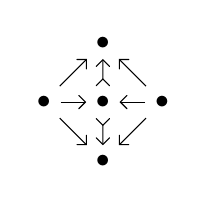
\begin{tikzpicture}[baseline=(current bounding box.center),scale=0.75]
		\node (A) at (0,0) {$\bullet$};
		\node (B) at (1,1) {$\bullet$};
		\node (B') at (1,0) {$\bullet$};
		\node (B'') at (1,-1) {$\bullet$};
		\node (C) at (2,0) {$\bullet$};
		%
		\path[->,font=\scriptsize,>=angle 90]
		(A) edge node[above]{$ $} (B)
		(A) edge node[above]{$ $} (B')
		(A) edge node[above]{$ $} (B'')
		(C) edge node[above]{$ $} (B)
		(C) edge node[above]{$ $} (B')
		(C) edge node[left]{$ $} (B'')
		(B') edge[>->] node[right]{$ $} (B)
		(B') edge[>->] node[left]{$ $} (B'');
		\end{tikzpicture}$ &
		% monic spans of cospans double category
		$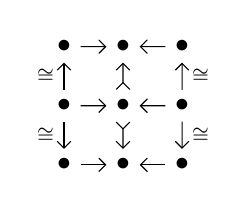
\begin{tikzpicture}[baseline=(current bounding box.center),scale=0.75]
		\node (A) at (0,2) {$\bullet$};
		\node (A') at (0,1) {$\bullet$};
		\node (A'') at (0,0) {$\bullet$};
		\node (B) at (1,2) {$\bullet$};
		\node (B') at (1,1) {$\bullet$};
		\node (B'') at (1,0) {$\bullet$};
		\node (C) at (2,2) {$\bullet$};
		\node (C') at (2,1) {$\bullet$};
		\node (C'') at (2,0) {$\bullet$};
		%
		\path[->,font=\scriptsize,>=angle 90]
		% horizontal arrows
		(A) edge node[above]{$ $} (B)
		(A') edge node[above]{$ $} (B')
		(A'') edge node[above]{$ $} (B'')
		(C) edge node[above]{$ $} (B)
		(C') edge node[above]{$ $} (B')
		(C'') edge node[above]{$ $} (B'')
		% vertical arrows
		(A') edge node[left]{$\cong$} (A)
		(A') edge node[left]{$\cong$} (A'')
		(B') edge[>->] node[left]{$ $} (B)
		(B') edge[>->] node[left]{$ $} (B'')
		(C') edge node[right]{$\cong$} (C)
		(C') edge node[right]{$\cong$} (C'');
		\end{tikzpicture}$ \\
		% Row 7
		\hline 
		{Epic Cospans of Spans} & 
		% epic cospans of spans bicategory
		$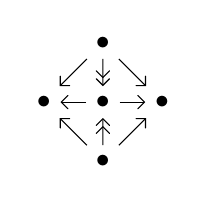
\begin{tikzpicture}[baseline=(current bounding box.center),scale=0.75]
		\node (A) at (0,0) {$\bullet$};
		\node (B) at (1,1) {$\bullet$};
		\node (B') at (1,0) {$\bullet$};
		\node (B'') at (1,-1) {$\bullet$};
		\node (C) at (2,0) {$\bullet$};
		%
		\path[->,font=\scriptsize,>=angle 90]
		(B) edge node[above]{$ $} (A)
		(B) edge node[left]{$ $} (C)
		(B') edge node[left]{$ $} (A)
		(B') edge node[right]{$ $} (C)
		(B'') edge node[left]{$ $} (A)
		(B'') edge node[left]{$ $} (C)
		(B) edge[->>] node[left]{$ $} (B')
		(B'') edge[->>] node[right]{$ $} (B');
		\end{tikzpicture}$ &
		% epic cospans of spans double category
		$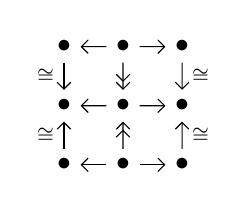
\begin{tikzpicture}[baseline=(current bounding box.center),scale=0.75]
		\node (A) at (0,2) {$\bullet$};
		\node (A') at (0,1) {$\bullet$};
		\node (A'') at (0,0) {$\bullet$};
		\node (B) at (1,2) {$\bullet$};
		\node (B') at (1,1) {$\bullet$};
		\node (B'') at (1,0) {$\bullet$};
		\node (C) at (2,2) {$\bullet$};;
		\node (C') at (2,1) {$\bullet$};
		\node (C'') at (2,0) {$\bullet$};
		%
		\path[->,font=\scriptsize,>=angle 90]
		% horizontal arrows
		(B) edge node[above]{$ $} (A)
		(B) edge node[above]{$ $} (C)
		(B') edge node[above]{$ $} (A')
		(B') edge node[above]{$ $} (C')
		(B'') edge node[above]{$ $} (A'')
		(B'') edge node[above]{$ $} (C'')
		% vertical arrows
		(A) edge node[left]{$\cong$} (A')
		(A'') edge node[left]{$\cong$} (A')
		(B) edge[->>] node[left]{$ $} (B')
		(B'') edge[->>] node[left]{$ $} (B')
		(C) edge node[right]{$\cong$} (C')
		(C'') edge node[right]{$\cong$} (C');
		\end{tikzpicture}$ \\
		\hline 
	\end{tabular}
	\caption{Bicategory and double category $2$-morphisms}
	\label{fig:2cells}
\end{figure}
The bicategory $\bicspmap{D}$, 
introduced by B\'enabou in his landmark paper \cite{Be}, 
consists of 
$\cat{D}$-objects as objects, 
cospans in $\cat{D}$ as 1-morphisms, and 
maps of cospans as $2$-morphisms. 
Later, Stay showed that $\bicspmap{D}$ is a compact closed symmetric monoidal bicategory \cite{Stay}. In related work, the first listed author constructed a bicategory
where spans and cospans interplayed in the 2-morphisms
	\cite{Cic}. 
Namely, if $\cat{T}$ is a topos, 
there is a bicategory $\bimonspcsp{T}$ consisting of 
$\cat{T}$ objects as objects, 
cospans in $\cat{T}$ as morphisms, and 
isomorphism classes of monic spans of cospans as 2-morphisms. 
Here, the span legs are 
required to be monomorphisms. 
These 2-morphisms are depicted in Figure \ref{fig:2cells}. 
One might wonder whether requiring monic span legs is truly necessary,
or whether a more aesthetic result is possible; it was shown \cite{Cic} that this condition is indeed necessary. 

In this paper, we show that $\bimonspcsp{T}$ is a symmetric monoidal bicategory. The definition of a symmetric monoidal bicategory is long, 
and so checking every axiom by hand is time consuming. 
Luckily, Shulman 
	\cite{Shul} 
provides a less tedious process. 
The idea is to construct an `isofibrant pseudo double category' that restricts, 
in a suitable sense, to the symmetric monoidal bicategory that we are interested in.  
If this double category is symmetric monoidal, 
then the `restricted' bicategory will be symmetric monoidal as well.  
The advantage is that it is much easier to check that a double category is symmetric monoidal \cite{Shul} than it is to check that a bicategory is symmetric monoidal \cite{Stay}.

There is more nice structure to this bicategory, namely we prove that $\bimonspcsp{T}$ is compact closed.
Stay \cite{Stay} has defined a compact closed bicategory 
to be a symmetric monoidal bicategory in which every object has a dual. However, the details are more involved than in the 1-category case: he requires
that each object be part of a `coherent dual pair'.  

The primary motivation for constructing $\bimonspcsp{T}$ 
is the case where $\cat{T}$ is the topos $\cat{Graph}$ of directed graphs. 
This is used as a framework to study diagrammatic calculi 
of open graphs and their rewrites
	\cite{Cic, Cic_zx}.
In particular, $\bimonspcsp{Graph}$ has a 
compact closed sub-bicategory 
	$\cat{Rewrite}$ 
that is 1-full and 2-full on the edgeless graphs.  
In $\cat{Rewrite}$, the 1-morphisms model open graphs 
by using the legs of the cospans to specify the inputs and outputs. 
An example of such a morphism is this cospan of graphs:
\[
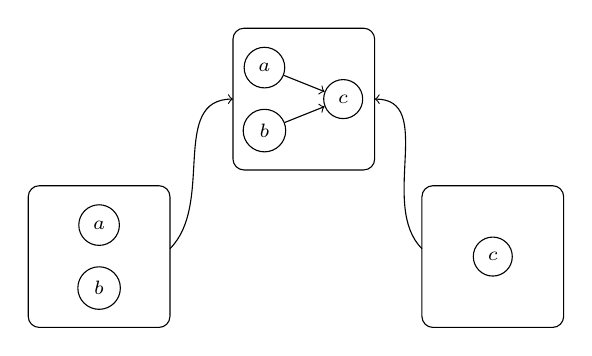
\begin{tikzpicture}[scale=1]
	\draw[rounded corners] (-0.8,1.6) rectangle (1,3.4);
	\draw[rounded corners] (4.2,1.6) rectangle (6,3.4);
	\draw[rounded corners] (1.8,3.6) rectangle (3.6,5.4);
	%
	\node[circle,draw] (ai) at (0.1,2.9) {\scriptsize $a$};
	\node[circle,draw] (bi) at (0.1,2.1) {\scriptsize $b$};
	\node[circle,draw] (co) at (5.1,2.5) {\scriptsize $c$};
	\node[circle,draw] (a1) at (2.2,4.9) {\scriptsize $a$};
	\node[circle,draw] (b1) at (2.2,4.1) {\scriptsize $b$};
	\node[circle,draw] (c1) at (3.2,4.5) {\scriptsize $c$};
	%
	\draw [->] (a1) edge (c1);
	\draw [->] (b1) edge (c1);
	%
	\path [->] (1,2.6) edge[out=45,in=180] (1.8,4.5);
	\path [->] (4.2,2.6) edge[out=135,in=0] (3.6,4.5);
\end{tikzpicture}
\]
The node labels indicate the graph morphism behavior. 
Here, the nodes $a$ and $b$ are inputs and $c$ is an output. 
The use of the terms \emph{inputs} and \emph{outputs} 
is justified by the composition,
which can be thought of as connecting the inputs of one graph
to compatible outputs of another graph. 
This is made precise with pushouts.  
For instance, we can compose
\[
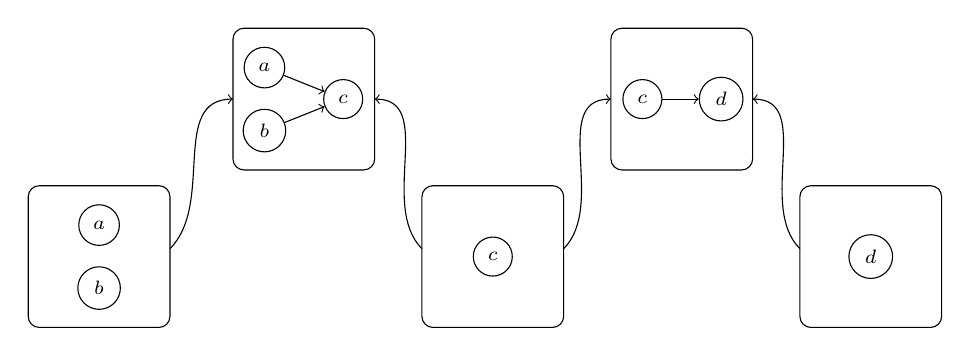
\begin{tikzpicture}[scale=1]
\draw[rounded corners] (-0.8,1.6) rectangle (1,3.4);
\draw[rounded corners] (1.8,3.6) rectangle (3.6,5.4);
\draw[rounded corners] (4.2,1.6) rectangle (6,3.4);
\draw[rounded corners] (6.6,3.6) rectangle (8.4,5.4);
\draw[rounded corners] (9,1.6) rectangle (10.8,3.4);
%
\node[circle,draw] (ai) at (0.1,2.9) {\scriptsize $a$};
\node[circle,draw] (bi) at (0.1,2.1) {\scriptsize $b$};
\node[circle,draw] (cm) at (5.1,2.5) {\scriptsize $c$};
\node[circle,draw] (a1) at (2.2,4.9) {\scriptsize $a$};
\node[circle,draw] (b1) at (2.2,4.1) {\scriptsize $b$};
\node[circle,draw] (c1) at (3.2,4.5) {\scriptsize $c$};
\node[circle,draw] (c2) at (7,4.5) {\scriptsize $c$};
\node[circle,draw] (d2) at (8,4.5) {\scriptsize $d$};
\node[circle,draw] (do) at (9.9,2.5) {\scriptsize $d$};
%
\draw [->] (a1) edge (c1);
\draw [->] (b1) edge (c1);
\draw [->] (c2) edge (d2);
%
\path [->] (1,2.6) edge[out=45,in=180] (1.8,4.5);
\path [->] (4.2,2.6) edge[out=135,in=0] (3.6,4.5);
\path [->] (6,2.6) edge[out=45,in=180] (6.6,4.5);
\path [->] (9,2.6) edge[out=135,in=0] (8.4,4.5);
\end{tikzpicture}
\]
to obtain
\[
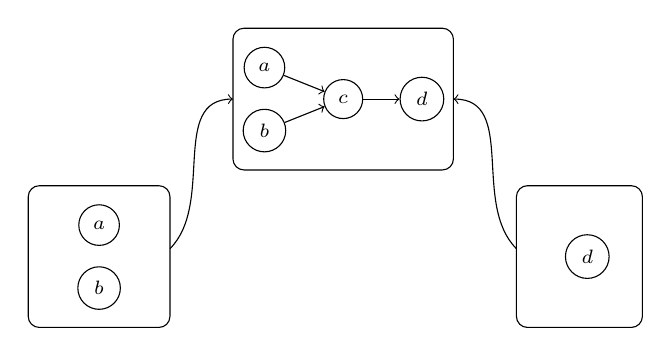
\begin{tikzpicture}[scale=1]
\draw[rounded corners] (-0.8,1.6) rectangle (1,3.4);
\draw[rounded corners] (1.8,3.6) rectangle (4.6,5.4);
\draw[rounded corners] (5.4,1.6) rectangle (7,3.4);
%
\node[circle,draw] (ai) at (0.1,2.9) {\scriptsize $a$};
\node[circle,draw] (bi) at (0.1,2.1) {\scriptsize $b$};
\node[circle,draw] (co) at (6.3,2.5) {\scriptsize $d$};
\node[circle,draw] (a1) at (2.2,4.9) {\scriptsize $a$};
\node[circle,draw] (b1) at (2.2,4.1) {\scriptsize $b$};
\node[circle,draw] (c1) at (3.2,4.5) {\scriptsize $c$};
\node[circle,draw] (d1) at (4.2,4.5) {\scriptsize $d$};
%
\draw [->] (a1) edge (c1);
\draw [->] (b1) edge (c1);
\draw [->] (c1) edge (d1);
%
\path [->] (1,2.6) edge[out=45,in=180] (1.8,4.5);
\path [->] (5.4,2.6) edge[out=135,in=0] (4.6,4.5);
\end{tikzpicture}
\]
A 2-morphism in $\cat{Rewrite}$ is the rewriting of one graph 
into another in a way that preserves inputs and outputs. 
For instance,
\begin{equation}
\label{diag:MonoidUnit}
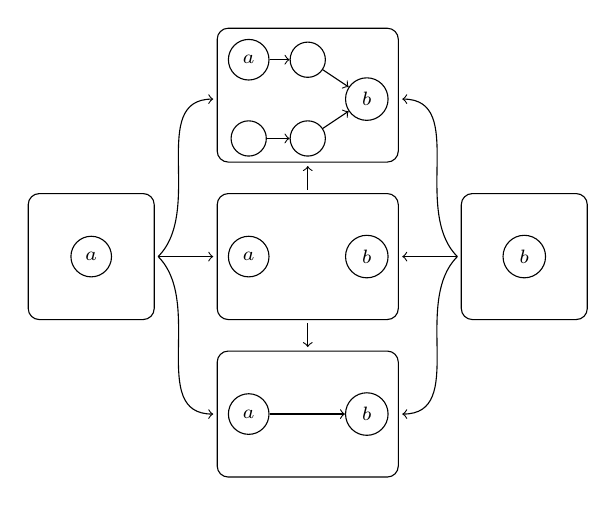
\begin{tikzpicture}[baseline=(current bounding box.center)]
	\draw[rounded corners] (1.6,-0.3) rectangle (3.9,1.3);
	\draw[rounded corners] (1.6,1.7) rectangle (3.9,3.3);
	\draw[rounded corners] (1.6,3.7) rectangle (3.9,5.4);
	\draw[rounded corners] (-0.8,1.7) rectangle (0.8,3.3);
	\draw[rounded corners] (4.7,1.7) rectangle (6.3,3.3);
	%
	\node[circle,draw] (ai) at (0,2.5) {\scriptsize $a$};
	\node[circle,draw] (bo) at (5.5,2.5) {\scriptsize $b$};
	\node[circle,draw] (a1) at (2,5) {\scriptsize $a$};
	\node[circle,draw,inner sep=4.5pt] (b1) at (2.75,5) {}; % unlabeled
	\node[circle,draw,inner sep=4.5pt] (c1) at (2,4) {}; % unlabeled
	\node[circle,draw,inner sep=4.5pt] (d1) at (2.75,4) {}; % unlabeled
	\node[circle,draw] (e1) at (3.5,4.5) {\scriptsize $b$};
	\node[circle,draw] (a2) at (2,2.5) {\scriptsize $a$};
	\node[circle,draw] (b2) at (3.5,2.5) {\scriptsize $b$};
	\node[circle,draw] (a3) at (2,0.5) {\scriptsize $a$};
	\node[circle,draw] (b3) at (3.5,0.5) {\scriptsize $b$};
	%
	\draw [->] (a1) edge (b1);
	\draw [->] (b1) edge (e1);
	\draw [->] (c1) edge (d1);
	\draw [->] (d1) edge (e1);
	\draw [->] (a3) edge (b3);
	%
	\path [->] (0.85,2.5) edge[out=0,in=180] (1.55,2.5);
	\path [->] (0.85,2.5) edge[out=45,in=180] (1.55,4.5);
	\path [->] (0.85,2.5) edge[out=-45,in=180] (1.55,0.5);
	\path [->] (4.65,2.5) edge[out=180,in=0] (3.95,2.5);
	\path [->] (4.65,2.5) edge[out=135,in=0] (3.95,4.5);
	\path [->] (4.65,2.5) edge[out=225,in=0] (3.95,0.5);
	\draw [->] (2.75,3.35) -- (2.75,3.65);
	\draw [->] (2.75,1.65) -- (2.75,1.35);
\end{tikzpicture}
\end{equation}
Actually, $\cat{Rewrite}$ is not entirely of interest in itself.
It serves as an ambient context in which to generate 
a compact closed bicategory 
from some collection of 1-morphisms and 2-morphisms. 
Of course, the choice of collection depends on one's interests.  
We illustrate this by considering 
the bicategory generated by a commutative Frobenius monoid. 
In this particular case, the diagram in \eqref{diag:MonoidUnit} then serves as the unit law.  
 
The structure of the paper is as follows.  
In Section 
	\ref{sec:Span cospan bicats}, 
we introduce the bicategory $\bimonspcsp{T}$.  
In Section 
	\ref{sec:DoubleCategories}, 
we review how double categories can be used 
to show that certain bicategories have a symmetric monoidal structure,
and moreover, when a symmetric monoidal bicategory is compact closed.  
Nothing in this section is new, but we use these results 
in Section \ref{sec:SpansCospans} 
to show that our bicategory is compact closed.
Finally, in Section 
	\ref{sec:Applications}, 
we discuss an application that uses $\bimonspcsp{Graph}$ to provide a bicategorical syntax  
for a category generated by a commutative monoid.

%%%%%%%%%%
%%%%%%%%%%
\section{The bicategory $\bold{MonicSp(Csp(T))}$} % EXAMPLES
\label{sec:Span cospan bicats}
%%%%%%%%%%
%%%%%%%%%%

In this section, we introduce the bicategory $\bimonspcsp{T}$.  
While this section contains nothing new, 
it does allow us to recall important concepts and to set our notation. 
Throughout this paper, 
$\cat{T}$ is a topos.

Spans of cospans were considered by Kissinger
in his thesis \cite{Kiss} in the context of rewriting,
and also by
Grandis and Par\'{e} 
	\cite{GranPare_Intercats} 
who found a lax interchange law. 
Later, the first listed author showed that the interchange law is invertible
	\cite{Cic} 
when restricting attention to a topos $\cat{T}$ and monic span legs. 
This gives a bicategory $\bimonspcsp{T}$ with 
$\cat{T}$-objects for objects, 
cospans for 1-morphisms, 
and isomorphism classes of monic spans of cospans for 2-morphisms. 
A monic span of cospans is a commuting diagram
\[
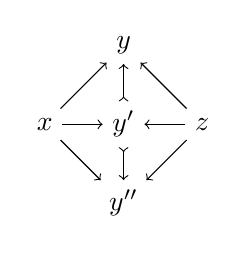
\begin{tikzpicture}[]
	\node (A) at (0,0) {$x$};
	\node (B) at (1,1) {$y$};
	\node (B') at (1,0) {$y'$};
	\node (B'') at (1,-1) {$y''$};
	\node (C) at (2,0) {$z$};
	%
	\path[->,font=\scriptsize]
	(A) edge node[above]{$ $} (B)
	(A) edge node[above]{$ $} (B')
	(A) edge node[above]{$ $} (B'')
	(C) edge node[above]{$ $} (B)
	(C) edge node[above]{$ $} (B')
	(C) edge node[left]{$ $} (B'')
	(B') edge[>->] node[right]{$ $} (B)
	(B') edge[>->] node[left]{$ $} (B'');
\end{tikzpicture}
\]
where the '$\rightarrowtail$' arrows denotes a monomorphism, and two of these are isomorphic if there is an isomorphism $\theta$ such that the following diagram commutes:
\[
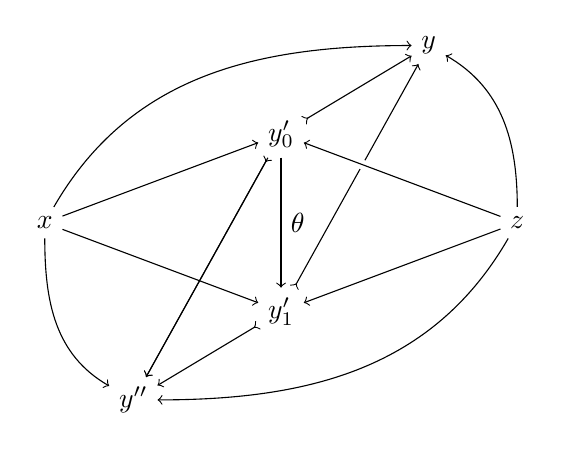
\begin{tikzpicture}[scale=1.5]
	\node (X) at (-2,0) {$x$};
	\node (L) at (1.25,1.5) {$y$};
	\node (Y) at (2,0) {$z$};
	\node (S) at (-1.25,-1.5) {$y''$};
	\node (S'1) at (0,0.75) {$y'_0$};
	\node (S'2) at (0,-0.75) {$y'_1$};
	%
	\draw [->] (X) edge[in=180,out=60] (L);
	\draw [->] (X) edge[] (S'1);
	\draw [->] (X) edge[] (S'2);
	\draw [->] (X) edge[out=-90,in=150] (S);
	\draw [->] (Y) edge[out=90,in=-30] (L);
	\draw [->] (Y) edge[] (S'2);
	\draw [->] (Y) edge[out=-120,in=0] (S);
	\draw [>->] (S'1) edge[] (L);
	%\draw [>->] (S'1) edge[white,line width=3.5pt] (S);
	\draw [>->] (S'1) edge[] (S);
	\draw [->] (S'1) edge[] (S);
	\draw [->] (S'1) edge node[right]{$\theta$} (S'2);
	\draw [>->] (S'2) edge[] (L);
	\draw [>->] (S'2) edge[] (S);
	\draw [->] (Y) edge[white,line width=3.5pt] (S'1);
	\draw [->] (Y) edge[] (S'1);
\end{tikzpicture}
\]
As usual, composition of morphisms is by pushout. Given vertically composable 2-morphisms
	\[
	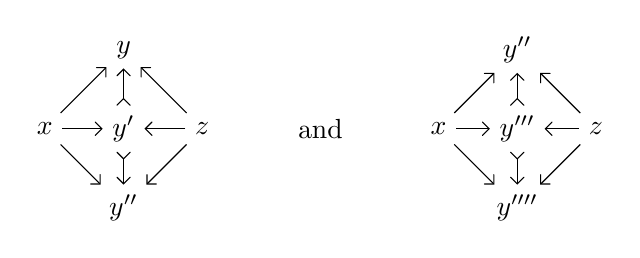
\begin{tikzpicture}
		\node (B) at (2,1) {$y$};
		\node (A') at (1,0) {$x$};
		\node (B') at (2,0) {$y^\prime$};
		\node (C') at (3,0) {$z$};
		\node (E) at (2,-1) {$y''$};
		
		
		\node (B'') at (7,1) {$y''$};

		\node (A''') at (6,0) {$x$};
		\node (B''') at (7,0) {$y'''$};
		\node (C''') at (8,0) {$z$};

		\node (E'') at (7,-1) {$y''''$};
		
		\node at (4.5,0) { and };
		%
		\path[->,font=\scriptsize,>=angle 90]
                     (C''') edge node {$$} (E'')
                     (A''') edge node {$$} (E'')
                     (C''') edge node {$$} (B'')
		(A''') edge node {$$} (B'')
                     (C') edge node {$$} (E)
                     (A') edge node {$$} (E)
                     (C') edge node [above]{$$}(B)
                     (A') edge node[above]{$$}(B)
                     (A') edge node[above]{$$}(B')
		(C')edge node[above]{$$}(B')
		(B') edge[>->] node[left]{$$} (B)
		
		(B') edge[>->] node[right]{$$} (E)
		
		
		
		(A''')edge node[above]{$$}(B''')
		(C''')edge node[above]{$$}(B''')
	
		
		(B''') edge[>->] node[left]{$$} (B'')
		
		
		(B''') edge[>->] node[right]{$$} (E'');
		
	\end{tikzpicture}
	\]
their vertical composite is given by
\[
	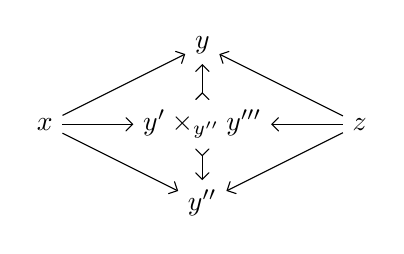
\begin{tikzpicture}
		\node (B) at (2,1) {$y$};
		\node (A') at (0,0) {$x$};
		\node (B') at (2,0) {$y^\prime \times_{y''} y'''$};
		\node (C') at (4,0) {$z$};
		\node (E) at (2,-1) {$y''$};
				%
		\path[->,font=\scriptsize,>=angle 90]
                   
                     (C') edge node {$$} (E)
                     (A') edge node {$$} (E)
                     (C') edge node [above]{$$}(B)
                     (A') edge node[above]{$$}(B)
                     (A') edge node[above]{$$}(B')
		(C')edge node[above]{$$}(B')
		(B') edge[>->] node[left]{$$} (B)
		(B') edge[>->] node[right]{$$} (E);
	\end{tikzpicture}
	\]
The legs of the inner span are monic because pullbacks preserve monomorphisms. Given two horizontally composable 2-morphisms
\[
	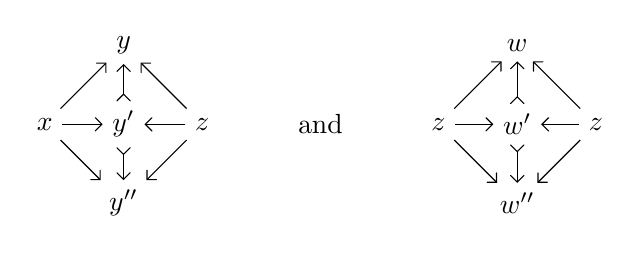
\begin{tikzpicture}
		\node (B) at (2,1) {$y$};
		\node (A') at (1,0) {$x$};
		\node (B') at (2,0) {$y^\prime$};
		\node (C') at (3,0) {$z$};
		\node (E) at (2,-1) {$y''$};
		
		
		\node (B'') at (7,1) {$w$};

		\node (A''') at (6,0) {$z$};
		\node (B''') at (7,0) {$w'$};
		\node (C''') at (8,0) {$z$};

		\node (E'') at (7,-1) {$w''$};
		
		\node at (4.5,0) { and };
		%
		\path[->,font=\scriptsize,>=angle 90]
                     (C''') edge node {$$} (E'')
                     (A''') edge node {$$} (E'')
                     (C''') edge node {$$} (B'')
		(A''') edge node {$$} (B'')
                     (C') edge node {$$} (E)
                     (A') edge node {$$} (E)
                     (C') edge node [above]{$$}(B)
                     (A') edge node[above]{$$}(B)
                     (A') edge node[above]{$$}(B')
		(C')edge node[above]{$$}(B')
		(B') edge[>->] node[left]{$$} (B)
		
		(B') edge[>->] node[right]{$$} (E)
		
		
		
		(A''')edge node[above]{$$}(B''')
		(C''')edge node[above]{$$}(B''')
	
		
		(B''') edge[>->] node[left]{$$} (B'')
		
		
		(B''') edge[>->] node[right]{$$} (E'');
		
	\end{tikzpicture}
	\]
their horizontal composite is given by
\[
	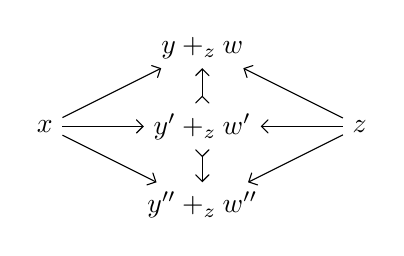
\begin{tikzpicture}
		\node (B) at (2,1) {$y+_z w$};
		\node (A') at (0,0) {$x$};
		\node (B') at (2,0) {$y^\prime +_z w^\prime$};
		\node (C') at (4,0) {$z$};
		\node (E) at (2,-1) {$y'' +_z w''$};
		
		
		
		%
		\path[->,font=\scriptsize,>=angle 90]
                   
                     (C') edge node {$$} (E)
                     (A') edge node {$$} (E)
                     (C') edge node [above]{$$}(B)
                     (A') edge node[above]{$$}(B)
                     (A') edge node[above]{$$}(B')
		(C')edge node[above]{$$}(B')
		(B') edge[>->] node[left]{$$} (B)
		
		(B') edge[>->] node[right]{$$} (E);
		
		
		
	\end{tikzpicture}
	\]
The legs of the inner span were previously showed to be monic \cite[Lem.~2.2]{Cic}. The monoidal structure is given by coproducts, and this again preserves the legs of the inner spans being monic.
	\[
	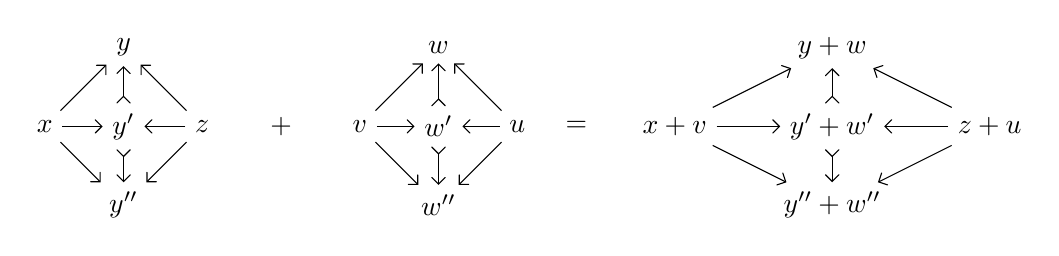
\begin{tikzpicture}
		\node (B) at (2,1) {$y$};
		\node (A') at (1,0) {$x$};
		\node (B') at (2,0) {$y^\prime$};
		\node (C') at (3,0) {$z$};
		\node (E) at (2,-1) {$y''$};
		
		
		\node (B'') at (6,1) {$w$};

		\node (A''') at (5,0) {$v$};
		\node (B''') at (6,0) {$w'$};
		\node (C''') at (7,0) {$u$};

		\node (E'') at (6,-1) {$w''$};
		
		\node at (4,0) {$+$};
                     \node at (7.75,0) {$=$};
                     \node (A) at (9,0) {$x+v$};
                     \node (C) at (11,1) {$y+w$};
                     \node (D) at (11,0) {$y^\prime + w^\prime$};
                     \node (F) at (11,-1) {$y'' + w''$};
                     \node (G) at (13,0) {$z+u$};
		%
		\path[->,font=\scriptsize,>=angle 90]
                     (A) edge node {$$} (C)
                     (A) edge node {$$} (D)
                     (A) edge node {$$} (F)
                     (D) edge [>->] node {$$} (C)
                     (D) edge [>->] node {$$} (F)
                     (G) edge node {$$} (C)
                     (G) edge node {$$} (D)
                     (G) edge node {$$} (F)
                     (C''') edge node {$$} (E'')
                     (A''') edge node {$$} (E'')
                     (C''') edge node {$$} (B'')
		(A''') edge node {$$} (B'')
                     (C') edge node {$$} (E)
                     (A') edge node {$$} (E)
                     (C') edge node [above]{$$}(B)
                     (A') edge node[above]{$$}(B)
                     (A') edge node[above]{$$}(B')
		(C')edge node[above]{$$}(B')
		(B') edge[>->] node[left]{$$} (B)
		
		(B') edge[>->] node[right]{$$} (E)
		
		
		
		(A''')edge node[above]{$$}(B''')
		(C''')edge node[above]{$$}(B''')
	
		
		(B''') edge[>->] node[left]{$$} (B'')
		
		
		(B''') edge[>->] node[right]{$$} (E'');
		
	\end{tikzpicture}
	\]

When convenient, we will denote a span 
$x \gets y \to z$ as 
$y \from x \tospan z$ and cospan 
$x \to y \gets z$ as 
$y \from x \tocospan z$.
This bicategory will be explored more in Section 
	\ref{subsec:Rewrite} 
where we take $\cat{T}$ to be the topos of directed graphs. 
There is also a dual bicategory $\biepiccspsp{T^{op}}$ with 
$\cat{T}$-objects for objects, 
spans for 1-morphisms, 
and isomorphism classes of epic cospans of spans for 2-morphisms. 

%%%%%%%%%%%%%%%%
%%%%%%%%%%%%%%%%
\section{Double categories and duality} % DOUBLE CATS AND DUALITY SECTION
\label{sec:DoubleCategories}
%%%%%%%%%%%%%%%%
%%%%%%%%%%%%%%%%

Bicategories are nice, 
but symmetric monoidal bicategories are much nicer.
Unfortunately, checking the axioms 
for a symmetric monoidal bicategory 
is daunting due to the sheer quantity of them.  
However, using a result of Shulman 
	\cite{Shul}, 
we can circumvent checking the axioms by, instead, 
promoting our bicategories to double categories 
and showing that the double categories are symmetric monoidal.  
This involves proving that a pair of categories are symmetric monoidal, 
which is a much more manageable task.  
Better than symmetric monoidal bicategories 
are those that are compact closed. 
The notion of compact closedness
we consider was given by Stay \cite{Stay}.
After summarizing Shulman's and Stay's work,
we will use their machinery
to show that $\bimonspcsp{T}$
is not only symmetric monoidal, but also compact closed.

%%%%%%%%%%%
%%%%%%%%%%%
\subsection{Monoidal bicategories via double categories}
\label{subsec:DoubleCategories}
%%%%%%%%%%%
%%%%%%%%%%%

Double categories, 
or pseudo-double categories to be precise, 
have been studied by Fiore 
	\cite{Fiore} 
and Par\'{e} and Grandis
	\cite{Gran} among others. 
Before giving a formal definition, 
it is helpful to have the following picture in mind. 
A double category has 2-morphisms that look like

\begin{equation}
\label{diag:DblCatSquare}
\raisebox{-0.5\height}{
	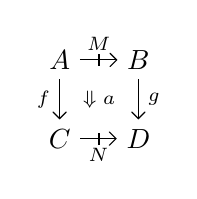
\begin{tikzpicture}
	\node (A) at (0,1) {$A$};
	\node (B) at (1,1) {$B$};
	\node (C) at (0,0) {$C$};
	\node (D) at (1,0) {$D$};
	%
	\path[->,font=\scriptsize,>=angle 90]
	(A) edge node[above]{$M$} (B)
	(A) edge node[left]{$f$} (C)
	(B) edge node[right]{$g$} (D)
	(C) edge node[below]{$N$} (D);
	%
	\draw (0.5,.925) -- (0.5,1.075);
	\draw (0.5,-.075) -- (0.5,.075);
	\node () at (0.5,0.5) {\scriptsize{$\Downarrow a$}};
	\end{tikzpicture}
}
\end{equation}
We call $A$, $B$, $C$ and $D$ \textbf{objects} or \textbf{0-cells}, 
$f$ and $g$ \textbf{vertical 1-morphisms}, 
$M$ and $N$ \textbf{horizontal 1-morphisms}, 
and $a$ a \textbf{2-morphism}. 
Note that vertical 1-morphisms go between objects
and a 2-morphisms between horizontal 1-morphisms. 
In our definitions, we denote a double category
with a bold font `$\dblcat{D}$' 
either as a stand-alone letter 
or as the first letter in a longer name.

% definition -- double category
%
\begin{defn}
	\label{def:DoubleCategory}
	A \textbf{pseudo-double category} $\dblcat{D}$, 
	or simply \textbf{double category}, consists of 
	a category of objects $\dblcat{D}_{0}$ and 
	a category of arrows $\dblcat{D}_{1}$ together
	with the following functors
	\begin{equation*}
		\begin{split}
			U & 
				\from \dblcat{D}_{0} \to \dblcat{D}_{1}, \\
			S,T & 
				\from \dblcat{D}_{1} \rightrightarrows \dblcat{D}_{0}, \t{ and} \\
			\odot & 
				\from \dblcat{D}_{1} \times_{\dblcat{D}_{0}} \dblcat{D}_{1} 
					\to \dblcat{D}_{1}
		\end{split}
	\end{equation*}
	where the pullback 
		$\dblcat{D}_{1} \times_{\dblcat{D}_{0}} \dblcat{D}_{1}$ 
	is taken over $S$ and $T$.  
	These functors satisfy the equations
	\begin{equation*}
		\begin{split}
			S(U_{A}) = A & = T(U_{A}) \\
			S(M \odot N) & = SN \\
			T(M \odot N) & = TM. 
	\end{split}
	\end{equation*}
	This also comes equipped with natural isomorphisms
	\begin{equation*}
		\begin{split}
		\alpha & \from (M \odot N) \odot P \to M \odot (N \odot P)\\
		\lambda & \from U_{B} \odot M \to M\\
		\rho & \from M \odot U_{A} \to M
	\end{split}
	\end{equation*}
	such that 
		$S(\alpha)$, 
		$S(\lambda)$, 
		$S(\rho)$, 
		$T(\alpha)$, 
		$T(\lambda)$, and 
		$T(\rho)$ 
	are each identities and that 
	the coherence axioms of a monoidal category are satisfied. 
	
	To match this definition with the more intuitive terms used, we say
	\textbf{vertical 1-morphisms} for the $\dblcat{D}_{0}$-morphisms,
	\textbf{horizontal 1-morphisms} \footnote{Sometimes the term \textbf{horizontal 1-cell} is used for these \cite{Shul}, and for good reason. A $(n \times 1)$-category consists of categories $\bold{D_i}$ for $0 \leq i \leq n$ where the objects of $\bold{D_i}$ are $i$-cells and the morphisms of $\bold{D_i}$ are vertical $i+1$-morphisms. A double category is then just a $(1 \times 1)$-category. From this perspective, `cells' are always objects with morphisms going between them.} for the $\dblcat{D}_{1}$-objects, and
	\textbf{2-morphisms} for the $\dblcat{D}_{1}$-morphisms. 
	As for notation, vertical and horizontal morphisms 
	are written with the arrows $\to$ and $\hto$, respectively, and 
	2-morphisms are drawn as in 
		\eqref{diag:DblCatSquare}.
\end{defn}

An equivalent perspective to this definition 
is that a double category is 
a category `weakly internal' to $\cat{Cat}$. 

To bypass checking that a bicategory is monoidal, 
we will instead need to check 
that a certain double category is monoidal. 
To define a monoidal double category, however, 
we need the notion of a \textbf{globular 2-morphism}.  
This is a 2-morphism whose 
source and target vertical 1-morphisms are identities.

% Definition -- Monoidal Double Category
%
\begin{defn}
	\label{def:MonoidalDoubleCategory}
	A \textbf{monoidal double category} is 
	a double category $\dblcat{D}$ 
	such that:
	\begin{enumerate}
		\item $\dblcat{D}_{0}$ and $\dblcat{D}_{1}$ 
			are both monoidal categories;
		\item if $I$ is the monoidal unit of $\dblcat{D}_{0}$, 
			then $U_I$ is the monoidal unit of $\dblcat{D}_{1}$;
		\item $S$ and $T$ are strict monoidal functors and 
			preserve the associativity and unit constraints;
		\item there are globular 2-isomorphisms
			\[ 
				\mathfrak{x} \from 
					(M_1 \otimes N_1) \odot (M_2 \otimes N_2) 
					\to 
					(M_1\odot M_2) \otimes (N_1\odot N_2)
			\]
			and
			\[
				\mathfrak{u} \from 
				U_{A \otimes B} 
				\to 
				(U_A \otimes U_B)
			\]
			expressing that $\odot$ and $U$ are monoidal;
		\item \label{diag:MonDblCat}
			the commuting diagrams 
			\[
			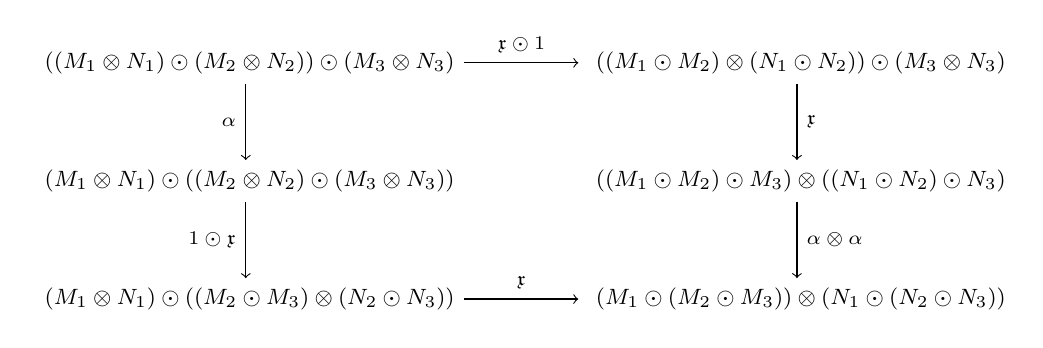
\begin{tikzpicture}
				\node (A) at (0,3) {\footnotesize{
							$((M_1\otimes N_1)\odot (M_2\otimes N_2)) \odot (M_3\otimes N_3)$}
				};
				\node (B) at (7,3) {\footnotesize{
						$((M_1\odot M_2)\otimes (N_1\odot N_2)) \odot (M_3\otimes N_3) $}
				};
				\node (A') at (0,1.5) {\footnotesize{
						$(M_1\otimes N_1)\odot ((M_2\otimes N_2) \odot (M_3\otimes N_3)) $}
				};
				\node (B') at (7,1.5) {\footnotesize{
						$((M_1\odot M_2)\odot M_3) \otimes ((N_1\odot N_2)\odot N_3)$}
				};
				\node (A'') at (0,0) {\footnotesize{
						$(M_1\otimes N_1) \odot ((M_2\odot M_3) \otimes (N_2\odot N_3))$}
				};
				\node (B'') at (7,0) {\footnotesize{
						$(M_1\odot (M_2\odot M_3)) \otimes (N_1\odot (N_2\odot N_3))$}
				};
			%
			\path[->,font=\scriptsize]
				(A) edge node[left]{$\alpha$} (A')
				(A') edge node[left]{$1 \odot \mathfrak{x}$} (A'')
				(B) edge node[right]{$\mathfrak{x}$} (B')
				(B') edge node[right]{$\alpha \otimes \alpha$} (B'')
				(A) edge node[above]{$\mathfrak{x} \odot 1$} (B)
				(A'') edge node[above]{$\mathfrak{x}$} (B'');
		\end{tikzpicture}
		\]
		\[
		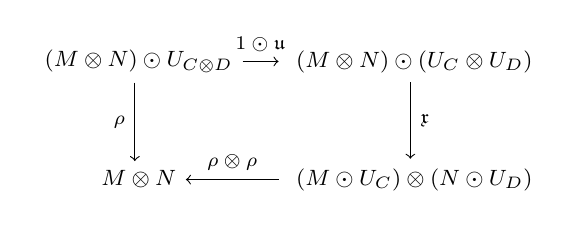
\begin{tikzpicture}
			\node (UL) at (0,1.5) {\footnotesize{
					$(M\otimes N) \odot U_{C\otimes D}$}
			};
			\node (LL) at (0,0) {\footnotesize{
					$M\otimes N$}
			};
			\node (UR) at (3.5,1.5) {\footnotesize{
					$(M\otimes N)\odot (U_C\otimes U_D)$}
			};
			\node (LR) at (3.5,0) {\footnotesize{
					$(M\odot U_C) \otimes (N\odot U_D)$}
			};
			%
			\path[->,font=\scriptsize]
				(UL) edge node[above]{$1 \odot \mathfrak{u}$} (UR) 
				(UL) edge node[left]{$\rho$} (LL)
				(LR) edge node[above]{$\rho \otimes \rho$} (LL)
				(UR) edge node[right]{$\mathfrak{x}$} (LR);
		\end{tikzpicture}
		%
		\quad
		%
		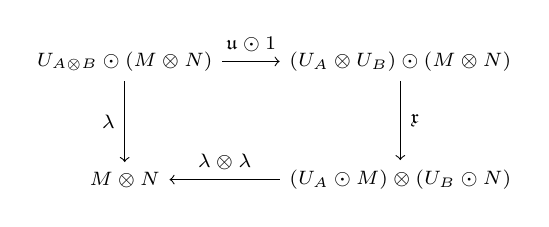
\begin{tikzpicture}
			\node (UL) at (0,1.5) {\scriptsize{$U_{A\otimes B}\odot (M\otimes N)$}};
			\node (LL) at (0,0) {\scriptsize{$M\otimes N$}};
			\node (UR) at (3.5,1.5) {\scriptsize{$(U_A\otimes U_B)\odot (M\otimes N)$}};
			\node (LR) at (3.5,0) {\scriptsize{$(U_A \odot M) \otimes (U_B\odot N)$}};
			%
			\path[->,font=\scriptsize]
				(UL) edge node[above]{$\mathfrak{u} \odot 1$} (UR) 
				(UL) edge node[left]{$\lambda$} (LL)
				(LR) edge node[above]{$\lambda \otimes \lambda$} (LL)
				(UR) edge node[right]{$\mathfrak{x}$} (LR);
		\end{tikzpicture}
		\]
		express the constraint data for the double functor $\otimes$;
		%
		\item the commuting diagrams expressing 
		the associativity isomorphism for $\otimes$ 
		\[
		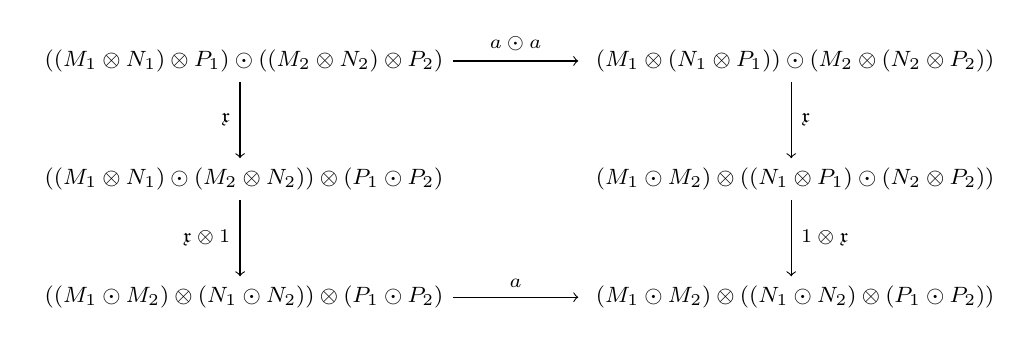
\begin{tikzpicture}
			\node (A) at (0,3) {\footnotesize{
					$((M_1\otimes N_1)\otimes P_1) \odot ((M_2\otimes N_2)\otimes P_2)$}
			};
			\node (B) at (7,3) {\footnotesize{
					$(M_1\otimes (N_1\otimes P_1)) \odot (M_2\otimes (N_2\otimes P_2))$}
			};
			\node (A') at (0,1.5) {\footnotesize{
					$((M_1\otimes N_1) \odot (M_2\otimes N_2)) \otimes (P_1\odot P_2)$}
			};
			\node (B') at (7,1.5) {\footnotesize{
					$(M_1\odot M_2) \otimes ((N_1\otimes P_1)\odot (N_2\otimes P_2))$}
			};
			\node (A'') at (0,0) {\footnotesize{
					$((M_1\odot M_2) \otimes(N_1\odot N_2)) \otimes (P_1\odot P_2)$}
			};
			\node (B'') at (7,0) {\footnotesize{
					$(M_1\odot M_2) \otimes ((N_1\odot N_2)\otimes (P_1\odot P_2))$}
			};
			%
			\path[->,font=\scriptsize]
				(A) edge node[left]{$\mathfrak{x}$} (A')
				(A') edge node[left]{$\mathfrak{x} \otimes 1$} (A'')
				(B) edge node[right]{$\mathfrak{x}$} (B')
				(B') edge node[right]{$1 \otimes \mathfrak{x}$} (B'')
				(A) edge node[above]{$a \odot a$} (B)
				(A'') edge node[above]{$a$} (B'');
		\end{tikzpicture}
		\]
		\[
		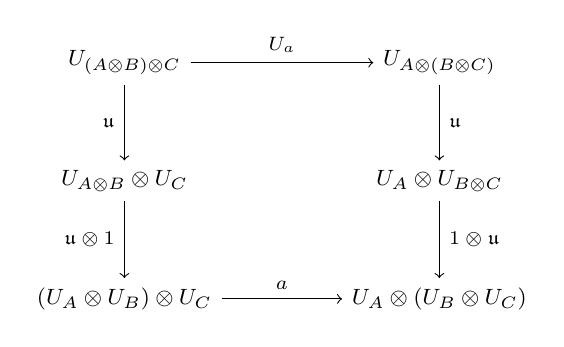
\begin{tikzpicture}
			\node (A) at (0,3) {\footnotesize{$U_{(A\otimes B)\otimes C}$}};
			\node (B) at (4,3) {\footnotesize{$U_{A\otimes (B\otimes C)} $}};
			\node (A') at (0,1.5) {\footnotesize{$U_{A\otimes B} \otimes U_C $}};
			\node (B') at (4,1.5) {\footnotesize{$U_A\otimes U_{B\otimes C}$}};
			\node (A'') at (0,0) {\footnotesize{$(U_A\otimes U_B)\otimes U_C$}};
			\node (B'') at (4,0) {\footnotesize{$U_A\otimes (U_B\otimes U_C) $}};
			%
			\path[->,font=\scriptsize]
				(A) edge node[left]{$\mathfrak{u}$} (A')
				(A') edge node[left]{$\mathfrak{u} \otimes 1$} (A'')
				(B) edge node[right]{$\mathfrak{u}$} (B')
				(B') edge node[right]{$1 \otimes \mathfrak{u}$} (B'')
				(A) edge node[above]{$U_{a}$} (B)
				(A'') edge node[above]{$a$} (B'');
		\end{tikzpicture}
		\]
		is a transformation of double categories;
		\item the commuting diagrams expressing that 
		the unit isomorphisms for $\otimes$ 
		\[
		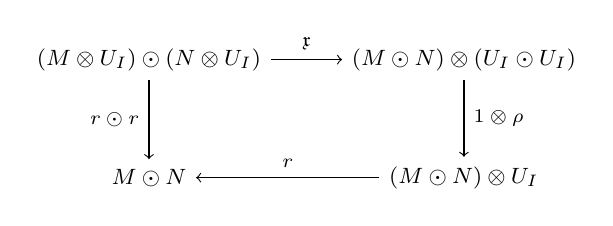
\begin{tikzpicture}
			\node (A) at (0,1.5) {\footnotesize{$(M\otimes U_I)\odot (N\otimes U_I)$}};
			\node (A') at (0,0) {\footnotesize{$M\odot N $}};
			\node (B) at (4,1.5) {\footnotesize{$(M\odot N)\otimes (U_I \odot U_I) $}};
			\node (B') at (4,0) {\footnotesize{$(M\odot N)\otimes U_I $}};
			%
			\path[->,font=\scriptsize]
				(A) edge node[left]{$r \odot r$} (A')
				(A) edge node[above]{$\mathfrak{x}$} (B)
				(B) edge node[right]{$1 \otimes \rho$} (B')
				(B') edge node[above]{$r$} (A');
		\end{tikzpicture}
		%
		\quad
		%
		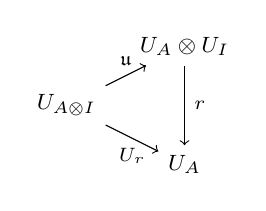
\begin{tikzpicture}
			\node (A) at (0,0.75) {\footnotesize{$U_{A\otimes I} $}};
			\node (B) at (1.5,1.5) {\footnotesize{$U_A\otimes U_I $}};
			\node (B') at (1.5,0) {\footnotesize{$U_A$}};
			%
			\path[->,font=\scriptsize]
				(A) edge node[above]{$\mathfrak{u}$} (B)
				(A) edge node[below]{$U_{r}$} (B')
				(B) edge node[right]{$r$} (B');
		\end{tikzpicture}
		\]
		%
		%
		%
		%
		\[
		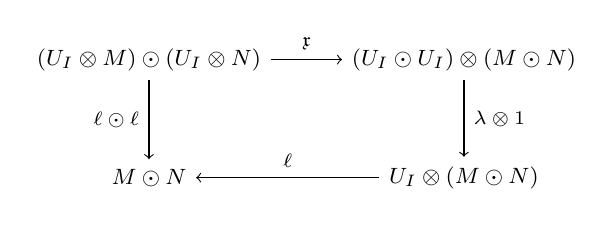
\begin{tikzpicture}
			\node (A) at (0,1.5) {\footnotesize{$(U_I\otimes M)\odot (U_I\otimes N)$}};
			\node (A') at (0,0) {\footnotesize{$M\odot N$}};
			\node (B) at (4,1.5) {\footnotesize{$(U_I \odot U_I) \otimes (M\odot N)$}};
			\node (B') at (4,0) {\footnotesize{$U_I\otimes (M\odot N) $}};
			%
			\path[->,font=\scriptsize]
				(A) edge node[left]{$\ell \odot \ell$} (A')
				(A) edge node[above]{$\mathfrak{x}$} (B)
				(B) edge node[right]{$\lambda \otimes 1$} (B')
				(B') edge node[above]{$\ell$} (A');
		\end{tikzpicture}
		%
		\quad
		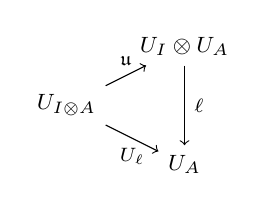
\begin{tikzpicture}
			\node (A) at (0,0.75) {\footnotesize{$U_{I\otimes A}$}};
			\node (B) at (1.5,1.5) {\footnotesize{$U_I\otimes U_A$}};
			\node (B') at (1.5,0) {\footnotesize{$U_A$}};
			%
			\path[->,font=\scriptsize]
				(A) edge node[above]{$\mathfrak{u}$} (B)
				(A) edge node[below]{$U_{\ell}$} (B')
				(B) edge node[right]{$\ell$} (B');
		\end{tikzpicture}
		\]
		are transformations of double categories.
		\newcounter{mondbl}
		\setcounter{mondbl}{\value{enumi}}
	\end{enumerate}
	A braided monoidal double category 
	is a monoidal double category 
	such that:
	\begin{enumerate}
		\setcounter{enumi}{\value{mondbl}}
		\item $\dblcat{D}_{0}$ and $\dblcat{D}_{1}$ are braided monoidal categories;
		\item $S$ and $T$ are strict braided monoidal functors,
		\item the diagrams
		\[
		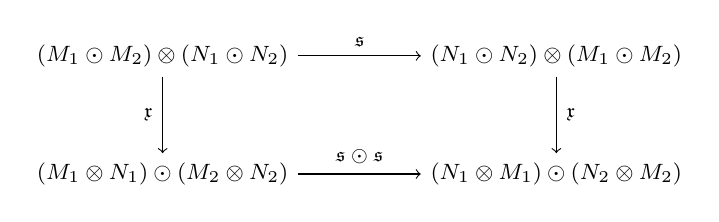
\begin{tikzpicture}
			\node (A) at (0,1.5) {\footnotesize{$(M_1 \odot M_2) \otimes (N_1 \odot N_2)$}};
			\node (A') at (0,0) {\footnotesize{$(M_1\otimes N_1) \odot (M_2\otimes N_2)$}};
			\node (B) at (5,1.5) {\footnotesize{$(N_1\odot N_2) \otimes (M_1 \odot M_2)$}};
			\node (B') at (5,0) {\footnotesize{$(N_1 \otimes M_1) \odot (N_2 \otimes M_2)$}};
			%
			\path[->,font=\scriptsize]
				(A) edge node[left]{$\mathfrak{x}$} (A')
				(A) edge node[above]{$\mathfrak{s}$} (B)
				(B) edge node[right]{$\mathfrak{x}$} (B')
				(A') edge node[above]{$\mathfrak{s} \odot \mathfrak{s}$} (B');
		\end{tikzpicture}
		%
		\quad
		%
		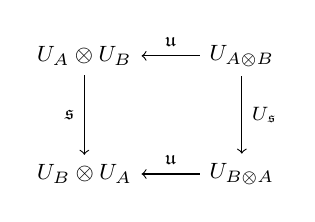
\begin{tikzpicture}
			\node (A) at (0,1.5) {\footnotesize{$U_A \otimes U_B$}};
			\node (A') at (0,0) {\footnotesize{$U_B\otimes U_A$}};
			\node (B) at (2,1.5) {\footnotesize{$U_{A\otimes B} $}};
			\node (B') at (2,0) {\footnotesize{$U_{B\otimes A}$}};
			%
			\path[->,font=\scriptsize]
				(A) edge node[left]{$\mathfrak{s}$} (A')
				(B) edge node[above]{$\mathfrak{u}$} (A)
				(B) edge node[right]{$U_\mathfrak{s}$} (B')
				(B') edge node[above]{$\mathfrak{u}$} (A');
		\end{tikzpicture}
		\]
		expressing that the braiding is a transformation of double categories commutes.
		\setcounter{mondbl}{\value{enumi}}
	\end{enumerate}
	Finally, a symmetric monoidal double category 
	is a braided monoidal double category $\mathbb{D}$ such that
	\begin{enumerate}
		\setcounter{enumi}{\value{mondbl}}
		\item $\dblcat{D}_{0}$ and $\dblcat{D}_{1}$ are symmetric monoidal.
	\end{enumerate}
\end{defn}

% DEFINITION -- Companion and Conjoint
%
\begin{defn}
	\label{def:CompanionConjoint}
	Let $\mathbb{D}$ be a double category and 
	$f \from A\to B$ a vertical 1-morphism.  
	A \textbf{companion} of $f$ is a horizontal 1-morphism
		$\widehat{f} \from A \hto B$ 
	together with 2-morphisms
	\[
	\raisebox{-0.5\height}{
	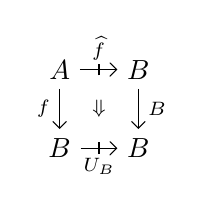
\begin{tikzpicture}
		\node (A) at (0,1) {$A$};
		\node (B) at (1,1) {$B$};
		\node (A') at (0,0) {$B$};
		\node (B') at (1,0) {$B$};
		%
		\path[->,font=\scriptsize,>=angle 90]
			(A) edge node[above]{$\widehat{f}$} (B)
			(A) edge node[left]{$f$} (A')
			(B) edge node[right]{$B$} (B')
			(A') edge node[below]{$U_B$} (B');
		%
		\draw (0.5,.925) -- (0.5,1.075);
		\draw (0.5,-.075) -- (0.5,.075);
		\node () at (0.5,0.5) {\scriptsize{$\Downarrow$}};
	\end{tikzpicture}
	}
	%
	\quad \text{ and } \quad
	%
	\raisebox{-0.5\height}{
	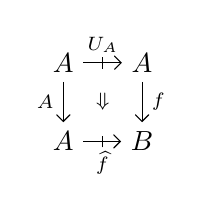
\begin{tikzpicture}
		\node (A) at (0,1) {$A$};
		\node (B) at (1,1) {$A$};
		\node (A') at (0,0) {$A$};
		\node (B') at (1,0) {$B$};
		%
		\path[->,font=\scriptsize,>=angle 90]
			(A) edge node[above]{$U_A$} (B)
			(A) edge node[left]{$A$} (A')
			(B) edge node[right]{$f$} (B')
			(A') edge node[below]{ $\widehat{f}$} (B');
		%
		\draw (0.5,.925) -- (0.5,1.075);
		\draw (0.5,-.075) -- (0.5,.075);
		\node () at (0.5,0.5) {\scriptsize{$\Downarrow$}};
	\end{tikzpicture}
	}
	\]
	such that the following equations hold:
	\begin{equation}
	\label{eq:CompanionEq}
	\raisebox{-0.5\height}{
	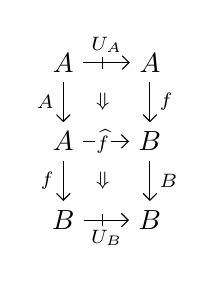
\begin{tikzpicture}
		\node (A) at (0,2) {$A$};
		\node (B) at (1.1,2) {$A$};
		\node (A') at (0,1) {$A$};
		\node (B') at (1.1,1) {$B$};
		\node (A'') at (0,0) {$B$};
		\node (B'') at (1.1,0) {$B$};
		%
		\path[->,font=\scriptsize,>=angle 90]
			(A) edge node[left]{$A$} (A')
			(A') edge node[left]{$f$} (A'')
			(B) edge node[right]{$f$} (B')
			(B') edge node[right]{$B$} (B'')
			(A) edge node[above]{$U_A$} (B)
			(A') edge  (B')
			(A'') edge node[below]{$U_B$} (B'');
		%
		\draw (0.5,1.925) -- (0.5,2.075);
		\draw[line width=2mm,white] (0.5,.925) -- (0.5,1.075);
		\draw (0.5,-.075) -- (0.5,.075);
		\node () at (0.5,0.5) {\scriptsize{$\Downarrow$}};
		\node () at (0.5,1.5) {\scriptsize{$\Downarrow$}};
		\node () at (0.5,1) {\scriptsize $\widehat{f}$};
	\end{tikzpicture}
	}
	%
	\raisebox{-0.5\height}{=}
	%
	\raisebox{-0.5\height}{
	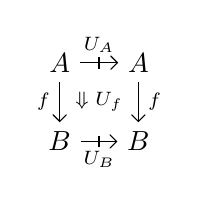
\begin{tikzpicture}
		\node (A) at (0,1) {$A$};
		\node (B) at (1,1) {$A$};
		\node (A') at (0,0) {$B$};
		\node (B') at (1,0) {$B$};
		%
		\path[->,font=\scriptsize,>=angle 90]
		(A) edge node[left]{$f$} (A')
		(B) edge node[right]{$f$} (B')
		(A) edge node[above]{$U_A$} (B)
		(A') edge node[below]{$U_B$} (B');
		%
		\draw (0.5,.925) -- (0.5,1.075);
		\draw (0.5,-.075) -- (0.5,.075);
		\node () at (0.5,0.5) {\scriptsize{$\Downarrow U_f$}};
	\end{tikzpicture}
	}
	%
	\raisebox{-0.5\height}{\text{   and   }}
	%
	\raisebox{-0.5\height}{
	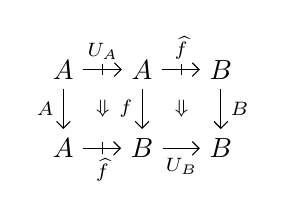
\begin{tikzpicture}
		\node (A) at (0,1) {$A$};
		\node (A') at (0,0) {$A$};
		\node (B) at (1,1) {$A$};
		\node (B') at (1,0) {$B$};
		\node (C) at (2,1) {$B$};
		\node (C') at (2,0) {$B$};
		%
		\path[->,font=\scriptsize,>=angle 90]
			(A) edge node[left]{$A$} (A')
			(B) edge node[left]{$f$} (B')
			(C) edge node[right]{$B$} (C')
			(A) edge node[above]{$U_A$} (B)
			(B) edge node[above]{$\widehat{f}$} (C)
			(A') edge node[below]{$\widehat{f}$} (B')
			(B') edge node[below]{$U_B$} (C');
		%
		\draw (1.5,0.925) -- (1.5,1.075);
		\draw (1.5,0.925) -- (1.5,1.075);
		\draw (0.5,.925) -- (0.5,1.075);
		\draw (0.5,-.075) -- (0.5,.075);
		\node () at (0.5,0.5) {\scriptsize{$\Downarrow$}};
		\node () at (1.5,0.5) {\scriptsize{$\Downarrow$}};
	\end{tikzpicture}
	}
	%
	\raisebox{-0.5\height}{=}
	%
	\raisebox{-0.5\height}{
	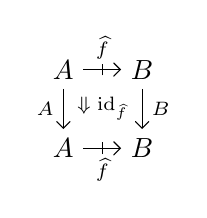
\begin{tikzpicture}
		\node (A) at (0,1) {$A$};
		\node (B) at (1,1) {$B$};
		\node (A') at (0,0) {$A$};
		\node (B') at (1,0) {$B$};
		%
		\path[->,font=\scriptsize,>=angle 90]
			(A) edge node[left]{$A$} (A')
			(B) edge node[right]{$B$} (B')
			(A) edge node[above]{$\widehat{f}$} (B)
			(A') edge node[below]{$\widehat{f}$} (B');
		%
		\draw (0.5,.925) -- (0.5,1.075);
		\draw (0.5,-.075) -- (0.5,.075);
		\node () at (0.5,0.5) {\scriptsize{$\Downarrow \id_{\widehat{f}}$}};
	\end{tikzpicture}
	}
	\end{equation}
	A \textbf{conjoint} of $f$, denoted 
		$\check{f} \from B \hto A$, 
	is a companion of $f$ in the double category 
		$\dblcat{D}^{h\cdot\mathrm{op}}$ 
	obtained by reversing the horizontal 1-cells, 
	but not the vertical 1-morphisms.
\end{defn}

% definition -- fibrant and isofibrant
%
\begin{defn}
	\label{def:Fibrant}
	We say that a double category is \textbf{fibrant} 
	if every vertical 1-morphism has 
	both a companion and a conjoint. 
	If every \emph{invertible} vertical 1-morphism 
	has both a companion and a conjoint, 
	then we say the double category is \textbf{isofibrant}.
\end{defn}

The final piece we need to present 
the main theorem of this section is the following.  
Given a double category $\dblcat{D}$, 
the \textbf{horizontal edge bicategory} 
	$H(\dblcat{D})$ 
of $\dblcat{D}$ is the bicategory whose 
objects are those of $\dblcat{D}$, 
morphisms are horizontal 1-morphisms of $\dblcat{D}$, 
and $2$-morphisms are the globular 2-morphisms.

\begin{thm}[Shulman {\cite[Theorem 5.1]{Shul}}]
	\label{thm:DoubleGivesBi}
	Let $\dblcat{D}$ be an isofibrant symmetric monoidal double category. 
	Then $H(\dblcat{D})$ is a symmetric monoidal bicategory.  
\end{thm}

Thanks to Theorem \ref{thm:DoubleGivesBi}, 
we can show that $\bimonspcsp{T}$
is symmetric monoidal
much more efficiently than
if we were to 
drudge through
all of the axioms.
But before we do show this,
we recall notions of compactness
is bicategories.

%%%%%%%%%%%%%%%
\subsection{Duality in bicategories}
\label{sec:CompactClosed}
%%%%%%%%%%%%%%%

In this section, we introduce various 
notions of duality in order to define
`compact closed bicategories' 
as conceived by Stay \cite{Stay}. 
We will suppress any notation 
for a monoidal operation and 
instead write $LR$ for the monoidal product 
of objects $L$ and $R$ and 
$fg$ for the monoidal product 
of morphisms $f$ and $g$.  
This will reserve the symbol `$\otimes$' 
for the horizontal composition functor 
of a bicategory.

\begin{defn}
	\label{def:DualPairCat}
	A \textbf{dual pair} in a monoidal category 
	is a tuple $(L,R,e,c)$ with objects $L$ and $R$, 
	called the left and right duals, 
	and morphisms
	\[
		e \from LR \to I 
		\quad \quad 
		c \from I \to RL,
	\]
	called evaluation and coevaluation such that the following diagams commute.
	\[
	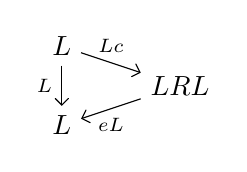
\begin{tikzpicture}
		\node (L1) at (0,1) {$L$};
		\node (L2) at (0,0) {$L$};
		\node (LRL) at (1.5,0.5) {$LRL$};
		%
		\path[->,font=\scriptsize,>=angle 90]
		(L1) edge node[left]{$L$} (L2)
		(L1) edge node[above]{$Lc$} (LRL)
		(LRL) edge node[below]{$eL$} (L2);
	\end{tikzpicture}
	%
	\quad \quad
	%
	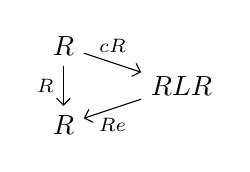
\begin{tikzpicture}
		\node (R1) at (0,1) {$R$};
		\node (R2) at (0,0) {$R$};
		\node (RLR) at (1.5,0.5) {$RLR$};
		%
		\path[->,font=\scriptsize,>=angle 90]
		(R1) edge node[left]{$R$} (R2)
		(R1) edge node[above]{$cR$} (RLR)
		(RLR) edge node[below]{$Re$} (R2);
	\end{tikzpicture}	
	\]
\end{defn}

\begin{defn}
	\label{def:DualPairBicat}
	A \textbf{dual pair} in a monoidal bicategory 
	is a tuple $(L,R,e,c,\alpha,\beta)$ with 
	objects $L$ and $R$, 
	morphisms
	\[
		e \from LR \to I 
		\quad \quad 
		c \from I \to RL,
	\]
	and invertible 2-morphisms
	\[
	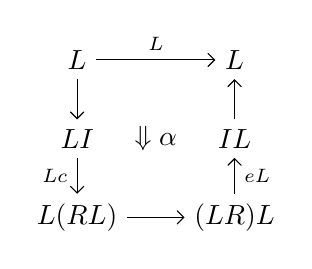
\begin{tikzpicture}
		\node (L1) at (0,2) {$L$};
		\node (LI) at (0,1) {$LI$};
		\node (LRL1) at (0,0) {$L(RL)$};
		\node (LRL2) at (2,0) {$(LR)L$};
		\node (IL) at (2,1) {$IL$};
		\node (L2) at (2,2) {$L$};
		%
		\path[->,font=\scriptsize,>=angle 90]
			(L1) edge (LI)
			(LI) edge node[left] {$Lc$} (LRL1)
			(LRL1) edge (LRL2)
			(LRL2) edge node[right] {$eL$} (IL)
			(IL) edge (L2)
			(L1) edge node[above] {$L$} (L2);
		%
		\node () at (1,1) {$\Downarrow \alpha$};
	\end{tikzpicture}
	%
	\quad \quad
	%
	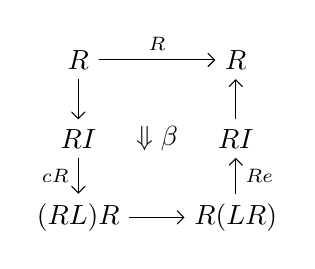
\begin{tikzpicture}
		\node (L1) at (0,2) {$R$};
		\node (LI) at (0,1) {$RI$};
		\node (LRL1) at (0,0) {$(RL)R$};
		\node (LRL2) at (2,0) {$R(LR)$};
		\node (IL) at (2,1) {$RI$};
		\node (L2) at (2,2) {$R$};
		%
		\path[->,font=\scriptsize,>=angle 90]
			(L1) edge (LI)
			(LI) edge node[left] {$cR$} (LRL1)
			(LRL1) edge (LRL2)
			(LRL2) edge node[right] {$Re$} (IL)
			(IL) edge (L2)
			(L1) edge node[above] {$R$} (L2);
		%
		\node () at (1,1) {$\Downarrow \beta$};
	\end{tikzpicture}
	\]
	called cusp isomorphisms.  
	If this data satisfies the swallowtail equations 
	in the sense that the diagrams in Figure 
		\ref{fig:Swallowtail} 
	are identities, 
	then we call the dual pair \textbf{coherent}.
\end{defn}

\begin{remark}
\label{rem:Swallowtail}
	To prevent cluttering in the diagrams in Figure 
		\ref{fig:Swallowtail}, 
	we will only write 
		$a$, $\rho$, and $\lambda$ 
	for the bicategory structure maps 
	even when we actually mean their inverse. 
\end{remark}

\begin{figure}[h]
	%
	%  DIAGRAM 1
	%
	\[
	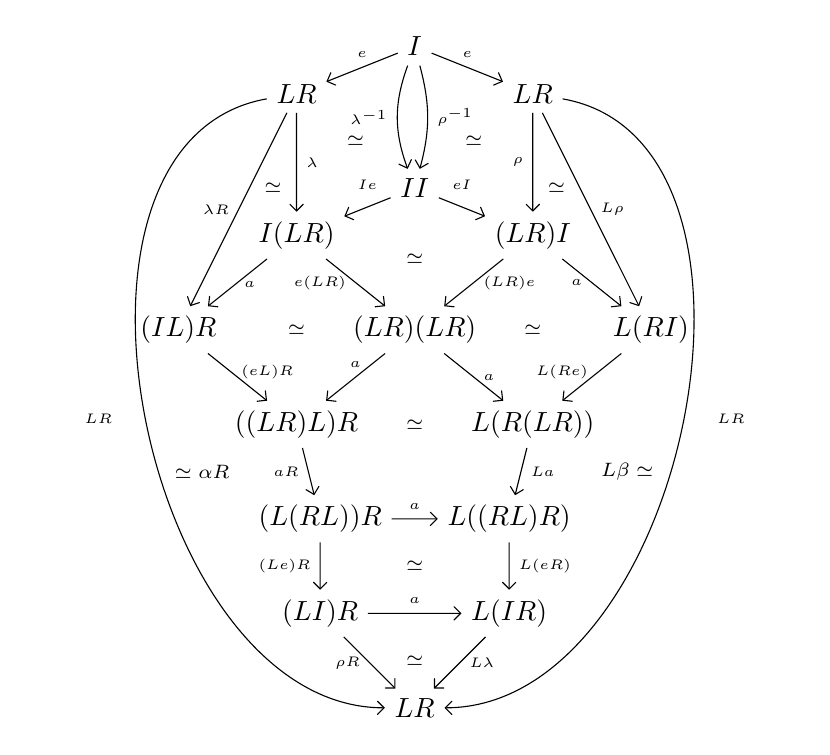
\begin{tikzpicture}[scale=0.60]
	\node (A) at (0,0) {$I$};
	\node (B) at (-2.5,-1) {$L R$};
	\node (C) at (2.5,-1) {$L R$};
	\node (D) at (0,-3) {$I I$};
	\node (E) at (-2.5,-4) {$I (L R)$};
	\node (F) at (2.5,-4) {$(L R) I$};
	\node (G) at (0,-6) {$(L R) (L R)$};
	\node (H) at (-5,-6) {$(I L) R$};
	\node (I) at (5,-6) {$L (R I)$};
	\node (J) at (-2.5,-8) {$((L R) L)  R$};
	\node (K) at (2.5,-8) {$L (R (L R))$};
	\node (L) at (-2,-10) {$(L (R L)) R$};
	\node (M) at (2,-10) {$L  ((R L) R)$};
	\node (N) at (-2,-12) {$(L I) R$};
	\node (O) at (2,-12) {$L (I R)$};
	\node (P) at (0,-14) {$L  R$};
	%
	%  2-CELLS
	%
	\node (Q) at (-1.25,-2) {\scriptsize{$\simeq$}};
	\node (R) at (1.25,-2) {\scriptsize{$\simeq$}};
	\node (S) at (0,-4.5) {\scriptsize{$\simeq$}};
	\node (T) at (-3,-3) {\scriptsize{$\simeq $}};
	\node (U) at (3,-3) {\scriptsize{$\simeq$}};
	\node (V) at (-2.5,-6) {\scriptsize{$\simeq$}};
	\node (W) at (2.5,-6) {\scriptsize{$\simeq$}};
	\node (X) at (0,-8) {\scriptsize{$\simeq$}};
	\node (Y) at (0,-11) {\scriptsize{$\simeq$}};
	\node (Z) at (0,-13) {\scriptsize{$\simeq$}};
	\node (A1) at (-4.5,-9) {\scriptsize{$\simeq \alpha R$}};
	\node (A2) at (4.5,-9) {\scriptsize{$L \beta \simeq$}};
	%
	\path[->,font=\tiny,>=angle 90]
	(A) edge node[above]{$e$} (B)
	(A) edge node[above]{$e$} (C)
	(A) edge[out=-110,in=110] node[left]{$\lambda^{-1}$} (D)
	(A) edge[out=-75,in=75] node[right]{$\rho^{-1}$} (D)
	(B) edge node[right]{$\lambda$}(E)
	(C) edge node[left]{$\rho$} (F)
	(D) edge node[left=0.2cm,above=0.1cm]{$I e$} (E)
	(D) edge node[left=0.2cm,above=0.1cm]{$e I$} (F)
	(E) edge node[below,left,pos=0.5]{$e (L R)$} (G)
	(F) edge node[below,right]{$(L R) e$} (G)
	(B) edge node[above,left]{$\lambda R$} (H)
	(C) edge node[above,right]{$L \rho$} (I)
	(E) edge node[below,right,pos=0.55]{$a$} (H)
	(F) edge node[below,left]{$a$} (I)
	(H) edge node[above,right,pos=0.4]{$(e L) R$} (J)
	(G) edge node[above]{$a$} (J)
	(I) edge node[above,left,pos=0.4]{$L (R e)$} (K)
	(G) edge node[above,right]{$a$} (K)
	(J) edge node[left]{$a R$} (L)
	(K) edge node[right]{$L a$} (M)
	(L) edge node[above]{$a$} (M)
	(L) edge node[left]{$(L  e) R$} (N)
	(M) edge node[right]{$L (e R)$} (O)
	(N) edge node[above]{$a$} (O)
	(N) edge node[below,left]{$\rho R$} (P)
	(O) edge node[below,right]{$L \lambda$} (P)
	(B) edge [out=-170,in=-180] node [below=0.3cm,left=0.3cm] {$L R$} (P)
	(C) edge [in=-360,out=-370,] node [below=0.3cm,right=0.3cm] {$LR$} (P);
	\end{tikzpicture}
	\]
	%
	%  DIAGRAM 2
	%
	\[
	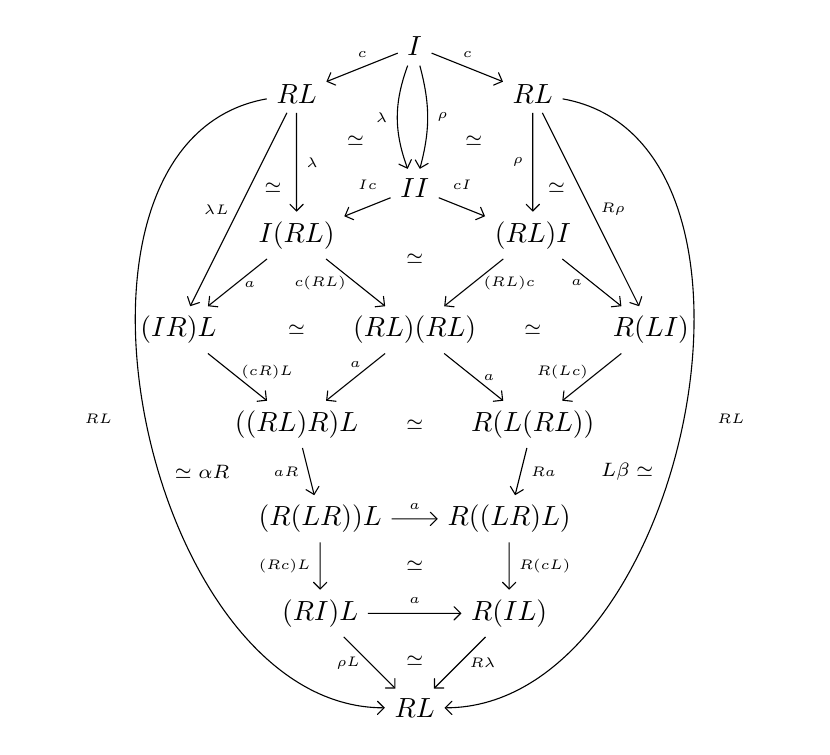
\begin{tikzpicture}[scale=0.60]
	\node (A) at (0,0) {$I$};
	\node (B) at (-2.5,-1) {$RL$};
	\node (C) at (2.5,-1) {$RL$};
	\node (D) at (0,-3) {$I I$};
	\node (E) at (-2.5,-4) {$I (RL)$};
	\node (F) at (2.5,-4) {$(RL) I$};
	\node (G) at (0,-6) {$(RL) (RL)$};
	\node (H) at (-5,-6) {$(I R) L$};
	\node (I) at (5,-6) {$R (L I)$};
	\node (J) at (-2.5,-8) {$((RL) R)  L$};
	\node (K) at (2.5,-8) {$R (L (R L))$};
	\node (L) at (-2,-10) {$(R (L R)) L$};
	\node (M) at (2,-10) {$R  ((L R) L)$};
	\node (N) at (-2,-12) {$(R I) L$};
	\node (O) at (2,-12) {$R (I L)$};
	\node (P) at (0,-14) {$R  L$};
	%
	%  2-CELLS
	%
	\node (Q) at (-1.25,-2) {\scriptsize{$\simeq$}};
	\node (R) at (1.25,-2) {\scriptsize{$\simeq$}};
	\node (S) at (0,-4.5) {\scriptsize{$\simeq$}};
	\node (T) at (-3,-3) {\scriptsize{$\simeq $}};
	\node (U) at (3,-3) {\scriptsize{$\simeq$}};
	\node (V) at (-2.5,-6) {\scriptsize{$\simeq$}};
	\node (W) at (2.5,-6) {\scriptsize{$\simeq$}};
	\node (X) at (0,-8) {\scriptsize{$\simeq$}};
	\node (Y) at (0,-11) {\scriptsize{$\simeq$}};
	\node (Z) at (0,-13) {\scriptsize{$\simeq$}};
	\node (A1) at (-4.5,-9) {\scriptsize{$\simeq \alpha R$}};
	\node (A2) at (4.5,-9) {\scriptsize{$L \beta \simeq$}};
	%
	\path[->,font=\tiny,>=angle 90]
	(A) edge[->] node[above]{$c$} (B)
	(A) edge[->] node[above]{$c$} (C)
	(A) edge[->,out=-110,in=110] node[left]{$\lambda$} (D)
	(A) edge[->,out=-75,in=75] node[right]{$\rho$} (D)
	(B) edge[->] node[right]{$\lambda$}(E)
	(C) edge[->] node[left]{$\rho$} (F)
	(D) edge[->] node[left=0.2cm,above=0.1cm]{$I c$} (E)
	(D) edge[->] node[left=0.2cm,above=0.1cm]{$c I$} (F)
	(E) edge[->] node[below,left,pos=0.5]{$c (R L)$} (G)
	(F) edge[->] node[below,right]{$(R L) c$} (G)
	(B) edge[->] node[above,left]{$\lambda L$} (H)
	(C) edge[->] node[above,right]{$R \rho$} (I)
	(E) edge[->] node[below,right,pos=0.55]{$a$} (H)
	(F) edge[->] node[below,left]{$a$} (I)
	(H) edge[->] node[above,right,pos=0.4]{$(c R) L$} (J)
	(G) edge[->] node[above]{$a$} (J)
	(I) edge[->] node[above,left,pos=0.4]{$R (L c)$} (K)
	(G) edge[->] node[above,right]{$a$} (K)
	(J) edge[->] node[left]{$a R$} (L)
	(K) edge[->] node[right]{$R a$} (M)
	(L) edge[->] node[above]{$a$} (M)
	(L) edge[->] node[left]{$(R  c) L$} (N)
	(M) edge[->] node[right]{$R (c L)$} (O)
	(N) edge[->] node[above]{$a$} (O)
	(N) edge[->] node[below,left]{$\rho L$} (P)
	(O) edge[->] node[below,right]{$R \lambda$} (P)
	(B) edge[->,out=-170,in=-180] node [below=0.3cm,left=0.3cm] {$R L$} (P)
	(C) edge[->,in=-360,out=-370] node [below=0.3cm,right=0.3cm] {$RL$} (P);
	\end{tikzpicture}
	\]
	\caption{The swallowtail diagrams for (co)evaluation}
	\label{fig:Swallowtail}
\end{figure}

Recall that a symmetric monoidal category is called 
\textbf{compact closed} if every object is part of a dual pair. 
We can generalize this idea to bicategories by 
introducing 2-morphisms and some coherence axioms. 
The following definition is due to Stay 
	\cite{Stay}.

\begin{defn}
	\label{def:CompClosdBicat}
	A \textbf{compact closed} bicategory is a symmetric monoidal bicategory for which
	every object $R$ 
	is part of a coherent dual pair. 
\end{defn}

The difference between showing compact closededness 
in categories versus bicategories might seem quite large 
because of the swallowtail equations.  
Looking at Figure 
	\ref{fig:Swallowtail}, 
it is no surprise that these can be incredibly tedious to work with.  
Fortunately, Pstragowski \cite{Piotr} proved a wonderful strictification theorem 
that effectively circumvents the need to consider the swallowtail equations.  

\begin{thm}[{\cite[p.~22]{Piotr}}]
	\label{thm:StrictingDualPairs}
	Given a dual pair $(L,R,e,c,\alpha,\beta)$, 
	we can find a cusp isomorphism $\beta'$ such that
	 $(L,R,e,c,\alpha,\beta')$ is a coherent dual pair.
\end{thm}

With the requisite background covered,
we can move on to our main results.

%%%%%%%%%%%%%%%%%%%%%%%%%%%%%%%%%%%%%%%%%%%%%%%%%%%%%%%%%%
%%%%%%%%%%%%%%%%%%%%%%%%%%%%%%%%%%%%%%%%%%%%%%%%%%%%%%%%%%
\section{Main results} % CSP & SPAN OF CSP
\label{sec:SpansCospans}
%%%%%%%%%%%%%%%%%%%%%%%%%%%%%%%%%%%%%%%%%%%%%%%%%%%%%%%%%%
%%%%%%%%%%%%%%%%%%%%%%%%%%%%%%%%%%%%%%%%%%%%%%%%%%%%%%%%%%

\begin{defn}
\label{def:DblCatMonSpanCsp}
	Let $\cat{T}$ be a topos. 
	We will define a double category 
		$\dblmonspcsp{T}$ 
	whose objects are the objects of $\bold{T}$
	vertical 1-morphisms are isomorphism classes of spans with invertible legs in $\bold{T}$, 
	horizontal 1-morphisms are cospans in $\bold{T}$, and 
	2-morphisms are isomorphism classes of spans of cospans in $\cat{T}$ with monic legs 
	(see Figure \ref{fig:2cells}). 
	We also have the double category $\dblepiccspsp{T}$, 
	which is defined dually to $\dblmonspcsp{T}$. 
\end{defn}

% DOUBLE CATEGORIES
\begin{lem}
\label{lem:SpanCospanDoubleCat}
	$\dblmonspcsp{T}$ is a double category.  
\end{lem}

\begin{proof}
	Denote $\dblmonspcsp{T}$ by $\dblcat{M}$.  
	The object category $\dblcat{M}_0$ is given by objects of $\bold{T}$ and spans in $\bold{T}$ such that each leg is an isomorphism. 
	The arrow category $\dblcat{M}_1$ has 
	as objects the cospans in $\bold{T}$ and 
	as morphisms the isomorphism classes of spans with monic legs 
	transversing the apexes of the cospans (see Figure \ref{fig:2cells}).  
	
	The structure functor 
		$U \from \dblcat{M}_0 \to \dblcat{M}_1$ 
	acts on objects by mapping $x$ to the identity cospan on $x$ and 
	on morphisms by mapping $y \from x \tospan z$, 
	whose legs are isomorphisms, 
	to the square
	\[
	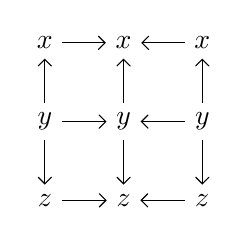
\begin{tikzpicture}
		\node (A) at (0,2) {$x$};
		\node (A') at (0,1) {$y$};
		\node (A'') at (0,0) {$z$};
		\node (B) at (1,2) {$x$};
		\node (B') at (1,1) {$y$};
		\node (B'') at (1,0) {$z$};
		\node (C) at (2,2) {$x$};
		\node (C') at (2,1) {$y$};
		\node (C'') at (2,0) {$z$};
		%
		\path[->,font=\scriptsize,>=angle 90]
		% horizontal arrows
		(A) edge node{} (B)
		(A') edge node{} (B')
		(A'') edge node{} (B'')
		(C) edge node{} (B)
		(C') edge node{} (B')
		(C'') edge node{} (B'')
		% vertical arrows
		(A') edge node{} (A)
		(A') edge node{} (A'')
		(B') edge node{} (B)
		(B') edge node{} (B'')
		(C') edge node{} (C)
		(C') edge node{} (C'');
	\end{tikzpicture}
	\]
	The structure functor 
		$S \from \dblcat{M}_1 \to \dblcat{M}_0$ 
	acts on objects by sending 
		$y \from x \tocospan z$ 
	to $x$ and on morphisms by sending 
	a square to the span occupying the  square's left vertical side.  
	The other functor $T$ is defined similarly.  
	
	The horizontal composition functor 
		$\odot \from \dblcat{M}_1 \times_{\dblcat{M}_0} \dblcat{M}_1 \to \dblcat{M}_1$ 
	acts on objects by composing cospans with pushouts in the usual way.  
	It acts on morphisms by 
	\[
	\raisebox{-0.5\height}{
		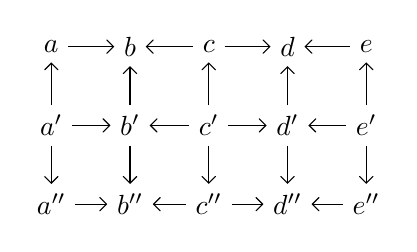
\begin{tikzpicture}
		\node (A) at (0,2) {$a$};
		\node (A') at (0,1) {$a'$};
		\node (A'') at (0,0) {$a''$};
		\node (B) at (1,2) {$b$};
		\node (B') at (1,1) {$b'$};
		\node (B'') at (1,0) {$b''$};
		\node (C) at (2,2) {$c$};
		\node (C') at (2,1) {$c'$};
		\node (C'') at (2,0) {$c''$};
		\node (D) at (3,2) {$d$};
		\node (D') at (3,1) {$d'$};
		\node (D'') at (3,0) {$d''$};
		\node (E) at (4,2) {$e$};
		\node (E') at (4,1) {$e'$};
		\node (E'') at (4,0) {$e''$};
		%
		\path[->,font=\scriptsize,>=angle 90]
		% horizontal arrows
		(A) edge node[above]{} (B)
		(A') edge node[above]{} (B')
		(A'') edge node[above]{} (B'')
		(C) edge node[above]{} (B)
		(C') edge node[above]{} (B')
		(C'') edge node[above]{} (B'')
		(C) edge node[above]{} (D)
		(C') edge node[above]{} (D')
		(C'') edge node[above]{} (D'')
		(E) edge node[above]{} (D)
		(E') edge node[above]{} (D')
		(E'') edge node[above]{} (D'')
		% vertical arrows
		(A') edge node[left]{} (A)
		(A') edge node[left]{} (A'')
		(B') edge node[left]{} (B)
		(B') edge node[left]{} (B'')
		(C') edge node[left]{} (C)
		(C') edge node[left]{} (C'')	
		(D') edge node[left]{} (D)
		(D') edge node[left]{} (D'')
		(E') edge node[left]{} (E)
		(E') edge node[left]{} (E'');
		\end{tikzpicture}
	}
	\quad
	\xmapsto[]{\odot}
	\quad
	\raisebox{-0.5\height}{
		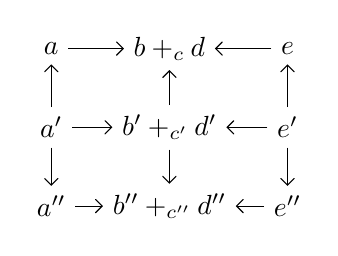
\begin{tikzpicture}
		\node (A) at (0,2) {$a$};
		\node (A') at (0,1) {$a'$};
		\node (A'') at (0,0) {$a''$};
		\node (B) at (1.5,2) {$b+_{c}d$};
		\node (B') at (1.5,1) {$b'+_{c'}d'$};
		\node (B'') at (1.5,0) {$b''+_{c''}d''$};
		\node (C) at (3,2) {$e$};
		\node (C') at (3,1) {$e'$};
		\node (C'') at (3,0) {$e''$};
		%
		\path[->,font=\scriptsize,>=angle 90]
		% horizontal arrows
		(A) edge node[above]{} (B)
		(A') edge node[above]{} (B')
		(A'') edge node[above]{} (B'')
		(C) edge node[above]{} (B)
		(C') edge node[above]{} (B')
		(C'') edge node[above]{} (B'')
		% vertical arrows
		(A') edge node[left]{} (A)
		(A') edge node[left]{} (A'')
		(B') edge node[left]{} (B)
		(B') edge node[left]{} (B'')
		(C') edge node[left]{} (C)
		(C') edge node[left]{} (C'');	
		\end{tikzpicture}
	}
	\]
	This respects identities. We prove that $\odot$ preserves
	composition in Lemma \ref{lem:InterchangeDblCat} below. 
	It is straightforward to check that the required equations are satisfied.  
	The associator and unitor natural isomorphisms arise from universal properties.  
\end{proof}

% INTERCHANGE LAW
\begin{lem}
\label{lem:InterchangeDblCat}
	The assignment $\odot$ from 
	Lemma \ref{lem:SpanCospanDoubleCat} 
	preserves composition. 
	In particular, $\odot$ is a functor.
\end{lem}

\begin{proof}
	Let $\alpha$, $\alpha^\prime$, $\beta$, and $\beta^\prime$ 
	be composable 2-morphisms given by
	\[
	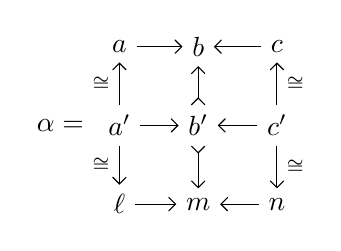
\begin{tikzpicture}
	\node () at (-0.75,1) {$\alpha =$};
	% nodes
	\node (A) at (0,2) {$a$};
	\node (A') at (0,1) {$a'$};
	\node (A'') at (0,0) {$\ell$};
	\node (B) at (1,2) {$b$};
	\node (B') at (1,1) {$b'$};
	\node (B'') at (1,0) {$m$};
	\node (C) at (2,2) {$c$};
	\node (C') at (2,1) {$c'$};
	\node (C'') at (2,0) {$n$};
	%
	\path[->,font=\scriptsize,>=angle 90]
	% horizontal arrows
	(A) edge node[above]{$$} (B)
	(A') edge node[above]{$$} (B')
	(A'') edge node[above]{$$} (B'')
	(C) edge node[above]{$$} (B)
	(C') edge node[above]{$$} (B')
	(C'') edge node[above]{$$} (B'')
	% vertical arrows
	(A') edge node[left]{$\cong$} (A)
	(A') edge node[left]{$\cong$} (A'')
	(B') edge[>->] node[left]{} (B)
	(B') edge[>->] node[left]{} (B'')
	(C') edge node[right]{$\cong$} (C)
	(C') edge node[right]{$\cong$} (C'');	
	\end{tikzpicture}
	%
	\quad \quad
	%
	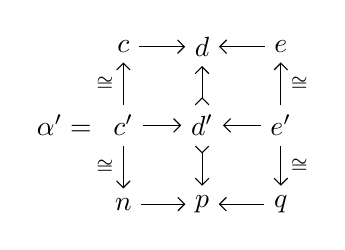
\begin{tikzpicture}
	\node () at (-0.75,1) {$\alpha' =$};
	% nodes
	\node (A) at (0,2) {$c$};
	\node (A') at (0,1) {$c'$};
	\node (A'') at (0,0) {$n$};
	\node (B) at (1,2) {$d$};
	\node (B') at (1,1) {$d'$};
	\node (B'') at (1,0) {$p$};
	\node (C) at (2,2) {$e$};
	\node (C') at (2,1) {$e'$};
	\node (C'') at (2,0) {$q$};
	%
	\path[->,font=\scriptsize,>=angle 90]
	% horizontal arrows
	(A) edge node[above]{$$} (B)
	(A') edge node[above]{$$} (B')
	(A'') edge node[above]{$$} (B'')
	(C) edge node[above]{$$} (B)
	(C') edge node[above]{$$} (B')
	(C'') edge node[above]{$$} (B'')
	% vertical arrows
	(A') edge node[left]{$\cong$} (A)
	(A') edge node[left]{$\cong$} (A'')
	(B') edge[>->] node[left]{} (B)
	(B') edge[>->] node[left]{} (B'')
	(C') edge node[right]{$\cong$} (C)
	(C') edge node[right]{$\cong$} (C'');	
	\end{tikzpicture}
	\]
	%
	%
	\[
	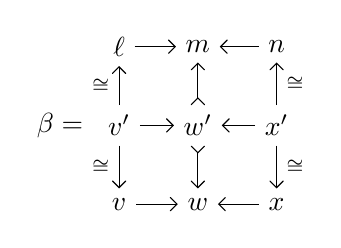
\begin{tikzpicture}
	\node () at (-0.75,1) {$\beta =$};
	% nodes
	\node (A) at (0,2) {$\ell$};
	\node (A') at (0,1) {$v'$};
	\node (A'') at (0,0) {$v$};
	\node (B) at (1,2) {$m$};
	\node (B') at (1,1) {$w'$};
	\node (B'') at (1,0) {$w$};
	\node (C) at (2,2) {$n$};
	\node (C') at (2,1) {$x'$};
	\node (C'') at (2,0) {$x$};
	%
	\path[->,font=\scriptsize,>=angle 90]
	% horizontal arrows
	(A) edge node[above]{$$} (B)
	(A') edge node[above]{$$} (B')
	(A'') edge node[above]{$$} (B'')
	(C) edge node[above]{$$} (B)
	(C') edge node[above]{$$} (B')
	(C'') edge node[above]{$$} (B'')
	% vertical arrows
	(A') edge node[left]{$\cong$} (A)
	(A') edge node[left]{$\cong$} (A'')
	(B') edge[>->] node[left]{} (B)
	(B') edge[>->] node[left]{} (B'')
	(C') edge node[right]{$\cong$} (C)
	(C') edge node[right]{$\cong$} (C'');	
	\end{tikzpicture}
	\quad \quad
	%
	%
	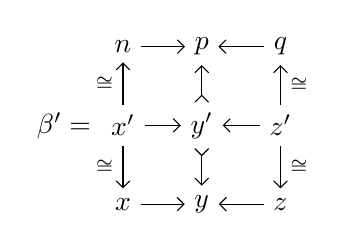
\begin{tikzpicture}
	\node () at (-0.75,1) {$\beta' =$};
	% nodes
	\node (A) at (0,2) {$n$};
	\node (A') at (0,1) {$x'$};
	\node (A'') at (0,0) {$x$};
	\node (B) at (1,2) {$p$};
	\node (B') at (1,1) {$y'$};
	\node (B'') at (1,0) {$y$};
	\node (C) at (2,2) {$q$};
	\node (C') at (2,1) {$z'$};
	\node (C'') at (2,0) {$z$};
	%
	\path[->,font=\scriptsize,>=angle 90]
	% horizontal arrows
	(A) edge node[above]{$$} (B)
	(A') edge node[above]{$$} (B')
	(A'') edge node[above]{$$} (B'')
	(C) edge node[above]{$$} (B)
	(C') edge node[above]{$$} (B')
	(C'') edge node[above]{$$} (B'')
	% vertical arrows
	(A') edge node[left]{$\cong$} (A)
	(A') edge node[left]{$\cong$} (A'')
	(B') edge[>->] node[left]{} (B)
	(B') edge[>->] node[left]{} (B'')
	(C') edge node[right]{$\cong$} (C)
	(C') edge node[right]{$\cong$} (C'');	
	\end{tikzpicture}
	\]
	Our goal is to show that
	\begin{equation}
	\label{eq:InterchangeCspSpan}
		(\alpha \odot \alpha') \circ (\beta \odot \beta')
		=
		(\alpha \circ \beta) \odot (\alpha' \circ \beta').
	\end{equation}
	The left hand side of \eqref{eq:InterchangeCspSpan} 
	corresponds to performing horizontal composition 
	before vertical composition. 
	The right hand side of \eqref{eq:InterchangeCspSpan} reverses that order.
	
	First, we compute the left hand side 
	of \eqref{eq:InterchangeCspSpan}. 
	Composing horizontally, 
	$\alpha \odot \alpha'$ and $\beta \odot \beta'$ 
	are, respectively,
	\[
	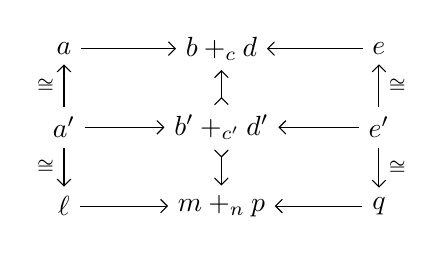
\begin{tikzpicture}
		\node (A) at (1,1) {$a$};
		\node (A') at (1,0) {$a'$};
		\node (A'') at (1,-1) {$\ell$};
		\node (B) at (3,1) {$b+_{c}d$};
		\node (B') at (3,0) {$b'+_{c'}d'$};
		\node (B'') at (3,-1) {$m+_{n}p$};
		\node (C) at (5,1) {$e$};
		\node (C') at (5,0) {$e'$};
		\node (C'') at (5,-1) {$q$};
		%
		\path[->,font=\scriptsize,>=angle 90]
		% horizontal arrows
		(A) edge node[above]{$$} (B)
		(A') edge node[above]{$$} (B')
		(A'') edge node[above]{$$} (B'')
		(C) edge node[above]{$$} (B)
		(C') edge node[above]{$$} (B')
		(C'') edge node[above]{$$} (B'')
		% vertical arrows
		(A') edge node[left]{$\cong$} (A)
		(A') edge node[left]{$\cong$} (A'')
		(B') edge[>->] node[left]{} (B)
		(B') edge[>->] node[left]{} (B'')
		(C') edge node[right]{$\cong$} (C)
		(C') edge node[right]{$\cong$} (C'');	
	\end{tikzpicture}
	%
	\quad \quad
	%
	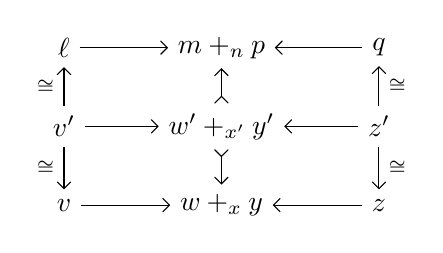
\begin{tikzpicture}
		\node (A) at (1,1) {$\ell$};
		\node (A') at (1,0) {$v'$};
		\node (A'') at (1,-1) {$v$};
		\node (B) at (3,1) {$m+_{n}p$};
		\node (B') at (3,0) {$w'+_{x'}y'$};
		\node (B'') at (3,-1) {$w+_{x}y$};
		\node (C) at (5,1) {$q$};
		\node (C') at (5,0) {$z'$};
		\node (C'') at (5,-1) {$z$};
		%
		\path[->,font=\scriptsize,>=angle 90]
		% horizontal arrows
		(A) edge node[above]{$$} (B)
		(A') edge node[above]{$$} (B')
		(A'') edge node[above]{$$} (B'')
		(C) edge node[above]{$$} (B)
		(C') edge node[above]{$$} (B')
		(C'') edge node[above]{$$} (B'')
		% vertical arrows
		(A') edge node[left]{$\cong$} (A)
		(A') edge node[left]{$\cong$} (A'')
		(B') edge[>->] node[left]{} (B)
		(B') edge[>->] node[left]{} (B'')
		(C') edge node[right]{$\cong$} (C)
		(C') edge node[right]{$\cong$} (C'');	
	\end{tikzpicture}
	\]
	The preservation of monics under 
	this operation follows from 
		\cite[Lem.~ 2.1]{Cic}.  
	Next, vertically composing 
	$\alpha \odot \alpha^\prime$ and 
	$\beta \odot \beta^\prime$, we get that 
	$(\alpha \odot \alpha^\prime) \circ (\beta \odot \beta^\prime)$ 
	is equal to
	\begin{equation}
	\label{diag:IntrchngHorVertCspSpan}
	\raisebox{-0.5\height}{
		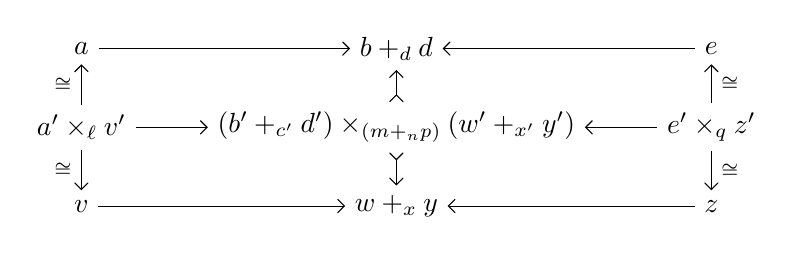
\begin{tikzpicture}
		\node (A) at (1,1) {$a$};
		\node (A') at (1,0) {$a'\times_{\ell}v'$};
		\node (A'') at (1,-1) {$v$};
		\node (B) at (5,1) {$b+_{d}d$};
		\node (B') at (5,0) {$(b'+_{c'}d') \times_{(m+_{n}p)} (w'+_{x'}y')$};
		\node (B'') at (5,-1) {$w+_{x}y$};
		\node (C) at (9,1) {$e$};
		\node (C') at (9,0) {$e' \times_{q}z'$};
		\node (C'') at (9,-1) {$z$};
		%
		\path[->,font=\scriptsize,>=angle 90]
		% horizontal arrows
		(A) edge node[above]{$$} (B)
		(A') edge node[above]{$$} (B')
		(A'') edge node[above]{$$} (B'')
		(C) edge node[above]{$$} (B)
		(C') edge node[above]{$$} (B')
		(C'') edge node[above]{$$} (B'')
		% vertical arrows
		(A') edge node[left]{$\cong$} (A)
		(A') edge node[left]{$\cong$} (A'')
		(B') edge[>->] node[left]{} (B)
		(B') edge[>->] node[left]{} (B'')
		(C') edge node[right]{$\cong$} (C)
		(C') edge node[right]{$\cong$} (C'');	
		\end{tikzpicture}
	}
	\end{equation}
	
	Solving for the right hand side 
	of \eqref{eq:InterchangeCspSpan}, 
	we first obtain that 
	$\alpha \circ \beta$ and $\alpha' \circ \beta'$ 
	are, respectively,
	\[
	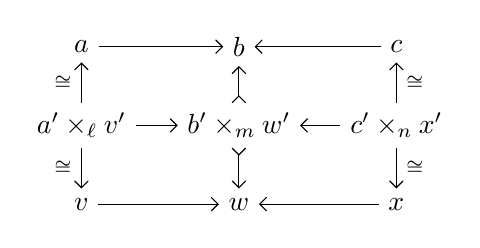
\begin{tikzpicture}
		\node (A) at (1,1) {$a$};
		\node (A') at (1,0) {$a' \times_{\ell}v'$};
		\node (A'') at (1,-1) {$v$};
		\node (B) at (3,1) {$b$};
		\node (B') at (3,0) {$b' \times_{m}w'$};
		\node (B'') at (3,-1) {$w$};
		\node (C) at (5,1) {$c$};
		\node (C') at (5,0) {$c' \times_{n}x'$};
		\node (C'') at (5,-1) {$x$};
		%
		\path[->,font=\scriptsize,>=angle 90]
		% horizontal arrows
		(A) edge node[above]{$$} (B)
		(A') edge node[above]{$$} (B')
		(A'') edge node[above]{$$} (B'')
		(C) edge node[above]{$$} (B)
		(C') edge node[above]{$$} (B')
		(C'') edge node[above]{$$} (B'')
		% vertical arrows
		(A') edge node[left]{$\cong$} (A)
		(A') edge node[left]{$\cong$} (A'')
		(B') edge[>->] node[left]{} (B)
		(B') edge[>->] node[left]{} (B'')
		(C') edge node[right]{$\cong$} (C)
		(C') edge node[right]{$\cong$} (C'');	
	\end{tikzpicture}
	%
	\quad \quad 
	%
	\begin{tikzpicture}
		\node (A) at (1,1) {$c$};
		\node (A') at (1,0) {$c' \times_{n}x'$};
		\node (A'') at (1,-1) {$x$};
		\node (B) at (3,1) {$d$};
		\node (B') at (3,0) {$d' \times_{p}y'$};
		\node (B'') at (3,-1) {$y$};
		\node (C) at (5,1) {$e$};
		\node (C') at (5,0) {$e' \times_{q}z'$};
		\node (C'') at (5,-1) {$z$};
		%
		\path[->,font=\scriptsize,>=angle 90]
		% horizontal arrows
		(A) edge node[above]{$$} (B)
		(A') edge node[above]{$$} (B')
		(A'') edge node[above]{$$} (B'')
		(C) edge node[above]{$$} (B)
		(C') edge node[above]{$$} (B')
		(C'') edge node[above]{$$} (B'')
		% vertical arrows
		(A') edge node[left]{$\cong$} (A)
		(A') edge node[left]{$\cong$} (A'')
		(B') edge[>->] node[left]{} (B)
		(B') edge[>->] node[left]{} (B'')
		(C') edge node[right]{$\cong$} (C)
		(C') edge node[right]{$\cong$} (C'');	
	\end{tikzpicture}
	\]
	Now composing these horizontally, 
	we get that 
	$(\alpha \circ \beta) \odot (\alpha^\prime \circ \beta^\prime)$ 
	equals
	\begin{equation}
	\label{diag:IntrchngVertHorCspSpan}
	\raisebox{-0.5\height}{
		\begin{tikzpicture}
		\node (A) at (1,1) {$a$};
		\node (A') at (1,0) {$a' \times_{\ell}v'$};
		\node (A'') at (1,-1) {$v$};
		\node (B) at (5,1) {$b +_{c}d$};
		\node (B') at (5,0) {$(b'\times_{m}w')+_{(c'\times_{n}x')}(d'\times_{p}y')$};
		\node (B'') at (5,-1) {$w+_{x}y$};
		\node (C) at (9,1) {$e$};
		\node (C') at (9,0) {$e' \times_{q}z'$};
		\node (C'') at (9,-1) {$z$};
		%
		\path[->,font=\scriptsize,>=angle 90]
		% horizontal arrows
		(A) edge node[above]{$$} (B)
		(A') edge node[above]{$$} (B')
		(A'') edge node[above]{$$} (B'')
		(C) edge node[above]{$$} (B)
		(C') edge node[above]{$$} (B')
		(C'') edge node[above]{$$} (B'')
		% vertical arrows
		(A') edge node[left]{$\cong$} (A)
		(A') edge node[left]{$\cong$} (A'')
		(B') edge[>->] node[left]{} (B)
		(B') edge[>->] node[left]{} (B'')
		(C') edge node[right]{$\cong$} (C)
		(C') edge node[right]{$\cong$} (C'');	
		\end{tikzpicture}
	}
	\end{equation}
	
	Now, we need to show that 
	\eqref{diag:IntrchngHorVertCspSpan} is equal to 
	\eqref{diag:IntrchngVertHorCspSpan} 
	as 2-morphisms.  
	Note that the diagrams only differ in the middle.  
	Thus, to complete the interchange law, 
	it suffices to establish an isomorphism 
	\[
		(b'+_{c'}d') \times_{(m+_{n}p)} (w'+_{x'}y')
		\to 
		(b' \times_{m}w')+_{(c' \times_{n}x')}(d' \times_{p}y')
	\]
	But because the left and right vertical spans 
	have isomorphisms for legs, 
	the isomorphism we seek follows from \cite[Lem.~2.5]{Cic}. 
\end{proof}


% DOUBLE CATEGORIES ARE SYMMETRIC MONOIDAL
\begin{lem}
\label{lem:SpanCospanSM}
	$\dblmonspcsp{T}$ is a symmetric monoidal double category.  
\end{lem}

\begin{proof}
	Let us first show that the category of objects 
		$\dblcat{M}_0$ 
	and the category of arrows 
		$\dblcat{M}_1$ 
	are symmetric monoidal.  
	Note that $\dblcat{M}_0$ is the 
	largest groupoid contained in $\bold{Sp(T)}$. 
	We obtain the monoidal structure on $\dblcat{M}_{0}$ by
	lifting the cocartesian structure on $\cat{T}$
	to the objects and by defining
	\[
		 (b \from a \tospan c) + (b' \from a' \tospan c')
		 =
		 (b+b' \from a+a' \tospan c+c')
	\]
	on morphisms.  
	Universal properties provide the 
	associator and unitors as well as 
	the coherence axioms. 
	This monoidal structure is clearly symmetric.
	
	Note that $\dblcat{M}_1$ is the category that has 
	as objects the cospans in $\cat{T}$ and 
	as morphisms the isomorphism classes of spans in $\cat{T}$.
	Moreover, the spans are required to have monic legs, 
	they go between apexes of cospans, 
	and they cause the evident diagrams to commute (see Figure \ref{fig:2cells}).  
	We obtain a symmetric monoidal structure on the objects via 
	\[
	(b \from a \tocospan c) + (b' \from a' \tocospan c')
	=
	(b+b' \from a+a' \tocospan c+c')
	\]
	and on the morphisms by
	\[
	\raisebox{-0.5\height}{
		\begin{tikzpicture}
		\node (A) at (0,2) {$\bullet$};
		\node (A') at (0,1) {$\bullet$};
		\node (A'') at (0,0) {$\bullet$};
		\node (B) at (1,2) {$\bullet$};
		\node (B') at (1,1) {$\bullet$};
		\node (B'') at (1,0) {$\bullet$};
		\node (C) at (2,2) {$\bullet$};
		\node (C') at (2,1) {$\bullet$};
		\node (C'') at (2,0) {$\bullet$};
		%
		\path[->,font=\scriptsize,>=angle 90]
		% horizontal arrows
		(A) edge node[above]{} (B)
		(A') edge node[above]{} (B')
		(A'') edge node[above]{} (B'')
		(C) edge node[above]{} (B)
		(C') edge node[above]{} (B')
		(C'') edge node[above]{} (B'')
		% vertical arrows
		(A') edge node[left]{} (A)
		(A') edge node[left]{} (A'')
		(B') edge[>->] node[left]{} (B)
		(B') edge[>->] node[left]{} (B'')
		(C') edge node[left]{} (C)
		(C') edge node[left]{} (C'');	
		\end{tikzpicture}
	}
	%
	\quad + \quad
	%
	\raisebox{-0.5\height}{
		\begin{tikzpicture}
		\node (A) at (0,2) {$\ast$};
		\node (A') at (0,1) {$\ast$};
		\node (A'') at (0,0) {$\ast$};
		\node (B) at (1,2) {$\ast$};
		\node (B') at (1,1) {$\ast$};
		\node (B'') at (1,0) {$\ast$};
		\node (C) at (2,2) {$\ast$};
		\node (C') at (2,1) {$\ast$};
		\node (C'') at (2,0) {$\ast$};
		%
		\path[->,font=\scriptsize,>=angle 90]
		% horizontal arrows
		(A) edge node[above]{} (B)
		(A') edge node[above]{} (B')
		(A'') edge node[above]{} (B'')
		(C) edge node[above]{} (B)
		(C') edge node[above]{} (B')
		(C'') edge node[above]{} (B'')
		% vertical arrows
		(A') edge node[left]{} (A)
		(A') edge node[left]{} (A'')
		(B') edge[>->] node[left]{} (B)
		(B') edge[>->] node[left]{} (B'')
		(C') edge node[left]{} (C)
		(C') edge node[left]{} (C'');	
		\end{tikzpicture}
	}
	%
	\quad = \quad
	%
	\raisebox{-0.5\height}{
		\begin{tikzpicture}
		\node (A) at (0,2) {$\bullet+\ast$};
		\node (A') at (0,1) {$\bullet+\ast$};
		\node (A'') at (0,0) {$\bullet+\ast$};
		\node (B) at (1.5,2) {$\bullet+\ast$};
		\node (B') at (1.5,1) {$\bullet+\ast$};
		\node (B'') at (1.5,0) {$\bullet+\ast$};
		\node (C) at (3,2) {$\bullet+\ast$};
		\node (C') at (3,1) {$\bullet+\ast$};
		\node (C'') at (3,0) {$\bullet+\ast$};
		%
		\path[->,font=\scriptsize,>=angle 90]
		% horizontal arrows
		(A) edge node[above]{} (B)
		(A') edge node[above]{} (B')
		(A'') edge node[above]{} (B'')
		(C) edge node[above]{} (B)
		(C') edge node[above]{} (B')
		(C'') edge node[above]{} (B'')
		% vertical arrows
		(A') edge node[left]{} (A)
		(A') edge node[left]{} (A'')
		(B') edge[>->] node[left]{} (B)
		(B') edge[>->] node[left]{} (B'')
		(C') edge node[left]{} (C)
		(C') edge node[left]{} (C'');	
		\end{tikzpicture}
	}
	\]
	Again, universal properties provide 
	the associator, unitors, and coherence axioms.  
	Hence both $\dblcat{M}_0$ and $\dblcat{M}_1$ 
	are symmetric monoidal categories.

It remains to find globular isomorphisms 
	for interchange $\mathfrak{x}$ 
	and units $\mathfrak{u}$ such that 
	the required diagrams commute. 
	To find $\mathfrak{x}$, fix horizontal morphisms 
	\begin{align*}
		b & \from a \tocospan c, & w &\from v \tocospan x, \\
		d & \from c \tocospan e, & y &\from x \tocospan z'.
	\end{align*}
	So $\mathfrak{x}$ is an invertible 2-morphism with domain
	\[
		(a+v) \to (b+w) +_{(c+x)} (d+y) \gets (e+z)
	\]
	and codomain
	\[
		(a+v) \to (b+_c d) + (w+_x y) \gets (e+z).
	\]
	This comes down to finding a isomorphism in $\bold{T}$ 
	between the apexes of the above cospans.  
	Such an isomorphism exists, and is unique, 
	because both apexes are colimits of the non-connected diagram
	\[
		\begin{tikzpicture}
			\node (a) at (0,0) {$a$};
			\node (b) at (1,.5) {$b$};
			\node (c) at (2,0) {$c$};
			\node (d) at (3,.5) {$d$};
			\node (e) at (4,0) {$e$};
			\node (v) at (5,0) {$v$};
			\node (w) at (6,.5) {$w$};
			\node (x) at (7,0) {$x$};
			\node (y) at (8,.5) {$y$};
			\node (z) at (9,0) {$z$};
			%
			\path[->,font=\scriptsize,>=angle 90]
			(a) edge node[above]{$$} (b)
			(c) edge node[above]{$$} (b)
			(c) edge node[above]{$$} (d)
			(e) edge node[above]{$$} (d)
			(v) edge node[above]{$$} (w)
			(x) edge node[above]{$$} (w)
			(x) edge node[above]{$$} (y)
			(z) edge node[above]{$$} (y);
		\end{tikzpicture}
	\]
	Moreover, the resulting globular isomorphism will be a monic span of cospans as the universal maps will be isomorphisms. The globular isomorphism $\mathfrak{u}$ is similar. Finally, we check that the coherence axioms, 
	namely (a)-(k) of Definition 
		\ref{def:MonoidalDoubleCategory}, 
	hold. 
	These are rather straightforward, though tedious, to verify. 
	For instance, if we have
	\[
		\begin{tikzpicture}
			\node (a) at (0,0) {$a$};
			\node (b) at (1,.5) {$b$};
			\node (c) at (2,0) {$c$};
			\node (M1) at (-1,.25) {$M_1 =$};
			\node (M2) at (3,.25) {$M_2 =$};
			\node (c2) at (4,0) {$c$};
			\node (d) at (5,.5) {$d$};
			\node (e) at (6,0) {$e$};
			\node (M3) at (7,.25) {$M_3 =$};
			\node (e2) at (8,0) {$e$};
			\node (f) at (9,.5) {$f$};
			\node (g) at (10,0) {$g$};
			\node (t) at (0,-2) {$t$};
			\node (u) at (1,-1.5) {$u$};
			\node (v) at (2,-2) {$v$};
			\node (N1) at (-1,-1.75) {$N_1 =$};
			\node (N2) at (3,-1.75) {$N_2 =$};
			\node (v2) at (4,-2) {$v$};
			\node (w) at (5,-1.5) {$w$};
			\node (x) at (6,-2) {$x$};
			\node (N3) at (7,-1.75) {$N_3 =$};
			\node (x2) at (8,-2) {$x$};
			\node (y) at (9,-1.5) {$y$};
			\node (z) at (10,-2) {$z$};
			%
			\path[->,font=\scriptsize,>=angle 90]
			(a) edge node[above]{$$} (b)
			(c) edge node[above]{$$} (b)
			(c2) edge node[above]{$$} (d)
			(e) edge node[above]{$$} (d)
			(v2) edge node[above]{$$} (w)
			(e2) edge node[above]{$$} (f)
			(g) edge node[above]{$$} (f)
			(t) edge node[above]{$$} (u)
			(v) edge node[above]{$$} (u)
			(x) edge node[above]{$$} (w)
			(x2) edge node[above]{$$} (y)
			(z) edge node[above]{$$} (y);
		\end{tikzpicture}
	\]
then following diagram \eqref{diag:MonDblCat} 
around the top right gives the sequence of cospans
\[
		\begin{tikzpicture}
			\node (a) at (-3,0) {$a+t$};
			\node (b) at (1,.5) {$((b+w)+_{c+v}(d+w))+_{e+x}(f+y)$};
			\node (c) at (5,0) {$g+z$};
			\node (M1) at (1,1.5) {$((M_1 \otimes N_1) \odot (M_2 \otimes N_2)) \odot (M_3 \otimes N_3) =$};
			%
			\path[->,font=\scriptsize]
			(a) edge[in=180,out=45] node[above]{$$} (b)
			(c) edge[in=0,out=135] node[above]{$$} (b);
		\end{tikzpicture}
	\]
	\[
		\begin{tikzpicture}
			\node (a) at (-3,0) {$a+t$};
			\node (b) at (1,.5) {$((b+_c d)+ (u+_v w))+_{e+x}(f+y)$};
			\node (c) at (5,0) {$g+z$};
			\node (M1) at (1,1.5) {$((M_1 \odot M_2) \otimes (N_1 \odot N_2)) \odot (M_3 \otimes N_3)=$};
			%
			\path[->,font=\scriptsize]
			(a) edge[in=180,out=45] node[above]{$$} (b)
			(c) edge[in=0,out=135] node[above]{$$} (b);
		\end{tikzpicture}
	\]
	\[
		\begin{tikzpicture}
			\node (a) at (-3,0) {$a+t$};
			\node (b) at (1,.5) {$((b+_c d)+_e f)+ ((u+_v w) +_x y)$};
			\node (c) at (5,0) {$g+z$};
			\node (M1) at (1,1.5) {$((M_1 \odot M_2) \odot M_3) \otimes ((N_1 \odot N_2) \odot N_3)=$};
			%
			\path[->,font=\scriptsize]
			(a) edge[in=180,out=45] node[above]{$$} (b)
			(c) edge[in=0,out=135] node[above]{$$} (b);
		\end{tikzpicture}
	\]
	\[
		\begin{tikzpicture}
			\node (a) at (-3,0) {$a+t$};
			\node (b) at (1,.5) {$(b+_c (d+_e f)) + (u+_v (w+_x y))$};
			\node (c) at (5,0) {$g+z$};
			\node (M1) at (1,1.5) {$(M_1 \odot (M_2 \odot M_3)) \otimes (N_1 \odot (N_2 \odot N_3)) =$};
			%
			\path[->,font=\scriptsize]
			(a) edge[in=180,out=45] node[above]{$$} (b)
			(c) edge[in=0,out=135] node[above]{$$} (b);
		\end{tikzpicture}
	\]
Following the diagram \eqref{diag:MonDblCat} 
around the bottom left gives another sequence of cospans
\[
		\begin{tikzpicture}
			\node (a) at (-3,0) {$a+t$};
			\node (b) at (1,.5) {$((b+w)+_{c+v}(d+w))+_{e+x}(f+y)$};
			\node (c) at (5,0) {$g+z$};
\node (M1) at (1,1.5) {$((M_1 \otimes N_1) \odot (M_2 \otimes N_2)) \odot (M_3 \otimes N_3) =$};
			%
			\path[->,font=\scriptsize]
			(a) edge[in=180,out=45] node[above]{$$} (b)
			(c) edge[in=0,out=135] node[above]{$$} (b);
		\end{tikzpicture}
	\]
\[
		\begin{tikzpicture}
			\node (a) at (-3,0) {$a+t$};
			\node (b) at (1,.5) {$(b+w)+_{c+v}((d+w)+_{e+x}(f+y))$};
			\node (c) at (5,0) {$g+z$};
\node (M1) at (1,1.5) {$(M_1 \otimes N_1) \odot ((M_2 \otimes N_2) \odot (M_3 \otimes N_3))=$};
			%
			\path[->,font=\scriptsize]
			(a) edge[in=180,out=45] node[above]{$$} (b)
			(c) edge[in=0,out=135] node[above]{$$} (b);
		\end{tikzpicture}
	\]
\[
		\begin{tikzpicture}
			\node (a) at (-3,0) {$a+t$};
			\node (b) at (1,.5) {$(b+u)+_{c+v}((d+_e f) + (w+_x y))$};
			\node (c) at (5,0) {$g+z$};
\node (M1) at (1,1.5) {$(M_1 \otimes N_1) \odot ((M_2 \odot M_3) \otimes (N_2 \odot N_3))=$};
			%
			\path[->,font=\scriptsize]
			(a) edge[in=180,out=45] node[above]{$$} (b)
			(c) edge[in=0,out=135] node[above]{$$} (b);
		\end{tikzpicture}
	\]
\[
		\begin{tikzpicture}
			\node (a) at (-3,0) {$a+t$};
			\node (b) at (1,.5) {$(b+_c (d+_e f)) + (u+_v (w+_x y))$};
			\node (c) at (5,0) {$g+z$};
\node (M1) at (1,1.5) {$(M_1 \odot (M_2 \odot M_3)) \otimes (N_1 \odot (N_2 \odot N_3)) =$};
			%
			\path[->,font=\scriptsize]
			(a) edge[in=180,out=45] node[above]{$$} (b)
			(c) edge[in=0,out=135] node[above]{$$} (b);
		\end{tikzpicture}
	\]
Putting this together gives the following commutative diagram.
\[
		\begin{tikzpicture}
			\node (a) at (-4,0) {$a+t$};
			\node (b) at (1,0) {$((b+w)+_{c+v}(d+w))+_{e+x}(f+y)$};
			\node (c) at (6,0) {$g+z$};
			\node (a2) at (-4,1.5) {$a+t$};
			\node (b2) at (1,1.5) {$((b+_c d)+ (u+_v w))+_{e+x}(f+y)$};
			\node (c2) at (6,1.5) {$g+z$};
                                \node (a3) at (-4,3) {$a+t$};
			\node (b3) at (1,3) {$((b+_c d)+_e f)+ ((u+_v w) +_x y)$};
			\node (c3) at (6,3) {$g+z$};
                                \node (a4) at (-4,4.5) {$a+t$};
			\node (b4) at (1,4.5) {$(b+_c (d+_e f)) + (u+_v (w+_x y))$};
			\node (c4) at (6,4.5) {$g+z$};
                                \node (a5) at (-4,-1.5) {$a+t$};
			\node (b5) at (1,-1.5) {$(b+w)+_{c+v}((d+w)+_{e+x}(f+y))$};
			\node (c5) at (6,-1.5) {$g+z$};
                                \node (a6) at (-4,-3) {$a+t$};
			\node (b6) at (1,-3) {$(b+u)+_{c+v}((d+_e f) + (w+_x y))$};
			\node (c6) at (6,-3) {$g+z$};
                                \node (a7) at (-4,-4.5) {$a+t$};
			\node (b7) at (1,-4.5) {$(b+_c (d+_e f)) + (u+_v (w+_x y))$};
			\node (c7) at (6,-4.5) {$g+z$};
			%
			\path[->,font=\scriptsize,>=angle 90]
			(a) edge node[above]{$$} (b)
			(c) edge node[above]{$$} (b)
                                (a2) edge node[above]{$$} (b2)
			(c2) edge node[above]{$$} (b2)
                                (a) edge node[above]{$$} (a2)
                                (b) edge node[above]{$$} (b2)
			(c) edge node[above]{$$} (c2)
                                (a3) edge node[above]{$$} (b3)
			(c3) edge node[above]{$$} (b3)
                                (a2) edge node[above]{$$} (a3)
                                (b2) edge node[above]{$$} (b3)
			(c2) edge node[above]{$$} (c3)
                                (a4) edge node[above]{$$} (b4)
			(c4) edge node[above]{$$} (b4)
                                (a3) edge node[above]{$$} (a4)
                                (b3) edge node[above]{$$} (b4)
			(c3) edge node[above]{$$} (c4)
                                (a5) edge node[above]{$$} (b5)
			(c5) edge node[above]{$$} (b5)
                                (a) edge node[above]{$$} (a5)
                                (b) edge node[above]{$$} (b5)
			(c) edge node[above]{$$} (c5)
                                (a6) edge node[above]{$$} (b6)
			(c6) edge node[above]{$$} (b6)
                                (a5) edge node[above]{$$} (a6)
                                (b5) edge node[above]{$$} (b6)
			(c5) edge node[above]{$$} (c6)
                                (a7) edge node[above]{$$} (b7)
			(c7) edge node[above]{$$} (b7)
                                (a6) edge node[above]{$$} (a7)
                                (b6) edge node[above]{$$} (b7)
			(c6) edge node[above]{$$} (c7);
		\end{tikzpicture}
	\]
 The vertical 1-morphisms on the left represent the identity span on $a+t$ and similarly for $g+z$ on the right. 
 The vertical 1-morphisms in the center represent isomorphism classes of monic spans where each leg is given by a universal map between two colimits of the same diagram and the horizontal 1-morphisms are given by universal maps into coproducts and pushouts.
 The top cospan is the same as the bottom cospan, 
 making a bracelet-like figure in which all faces commute.  
 The other diagrams witnessing coherence are given in a similar fashion.
	
\end{proof}

% DOUBLE CATEGORIES ARE ISOFIBRANT
\begin{lem}
\label{lem:SpanCospanIsofibrant}
	$\dblmonspcsp{T}$ is isofibrant.  
\end{lem}

\begin{proof}
	Take a vertical morphism 
		$f = (b \from a \tospan c)$ 
	whose legs are isomorphisms. 
	To get its companion 
		$\widehat{f} = (b \from a \tocospan c)$ 
	use the inverses of the legs of $f$, 
	and take the 2-morphisms
	\[
	\raisebox{-0.5\height}{
	\begin{tikzpicture}
		\node (A) at (0,2) {$a$};
		\node (A') at (0,1) {$b$};
		\node (A'') at (0,0) {$c$};
		\node (B) at (1,2) {$b$};
		\node (B') at (1,1) {$c$};
		\node (B'') at (1,0) {$c$};
		\node (C) at (2,2) {$c$};
		\node (C') at (2,1) {$c$};
		\node (C'') at (2,0) {$c$};
		%
		\path[->,font=\scriptsize,>=angle 90]
		% horizontal arrows
		(A) edge node[above]{} (B)
		(A') edge node[above]{} (B')
		(A'') edge node[above]{} (B'')
		(C) edge node[above]{} (B)
		(C') edge node[above]{} (B')
		(C'') edge node[above]{} (B'')
		% vertical arrows
		(A') edge node[left]{} (A)
		(A') edge node[left]{} (A'')
		(B') edge node[left]{} (B)
		(B') edge node[left]{} (B'')
		(C') edge node[left]{} (C)
		(C') edge node[left]{} (C'');
	\end{tikzpicture}
	}
	%
	\t{ and }
	%
	\raisebox{-0.5\height}{
	\begin{tikzpicture}
		\node (A) at (0,2) {$a$};
		\node (A') at (0,1) {$a$};
		\node (A'') at (0,0) {$a$};
		\node (B) at (1,2) {$a$};
		\node (B') at (1,1) {$a$};
		\node (B'') at (1,0) {$b$};
		\node (C) at (2,2) {$a$};
		\node (C') at (2,1) {$b$};
		\node (C'') at (2,0) {$c$};
		%
		\path[->,font=\scriptsize,>=angle 90]
		% horizontal arrows
		(A) edge node[above]{} (B)
		(A') edge node[above]{} (B')
		(A'') edge node[above]{} (B'')
		(C) edge node[above]{} (B)
		(C') edge node[above]{} (B')
		(C'') edge node[above]{} (B'')
		% vertical arrows
		(A') edge node[left]{} (A)
		(A') edge node[left]{} (A'')
		(B') edge node[left]{} (B)
		(B') edge node[left]{} (B'')
		(C') edge node[left]{} (C)
		(C') edge node[left]{} (C'');
	\end{tikzpicture}
	}
	\]
	The conjoint for $f$ is given by $\check{f} = \widehat{f}^{\text{op}}$.
\end{proof}

% BICATEEGORIES
\begin{thm}
	\label{thm:SpansCospasAreSMBicat}
	$\bimonspcsp{T}$ is a symmetric monoidal bicategory.
\end{thm}

\begin{proof}
	Apply Theorem \ref{thm:DoubleGivesBi} to $\mathbb{M} \bold{onicSp(Csp(T))}$ to obtain $\bold{MonicSp(Csp(T))}$.
\end{proof}

\begin{lem}
\label{lem:PushoutDiagram}
	The diagram
	\[
		\begin{tikzpicture}
			\node (UL) at (0,1) {$X+X+X$};
			\node (LL) at (0,0) {$X+X$};
			\node (UR) at (3,1) {$X+X$};
			\node (LR) at (3,0) {$X$};
			%
			\path[->,font=\scriptsize,>=angle 90]
			(UL) edge node[above] {$X+\nabla$} (UR)
			(UL) edge node[left] {$\nabla +X$} (LL)
			(UR) edge node[right] {$\nabla$} (LR)
			(LL) edge node[above] {$\nabla$} (LR);
		\end{tikzpicture}
	\]
	is a pushout square.
\end{lem}

\begin{proof}
	Suppose we have maps 
		$f,g \from X+X \to Y$
	forming a cocone over the span 
	inside the above diagram. 
	Let $\iota \from X \to X+X+X$ include $X$ 
	into the middle copy. 
	Observe that 
		$\ell \coloneqq (\nabla + X) \circ \iota$ 
	and 
		$r \coloneqq (X + \nabla) \circ \iota$ 
	are, respectively, the left and right inclusions 
		$X \to X+X$. 
	Then $f \circ \ell = g \circ r$ is a map $X \to Y$, 
	which we claim is the unique map making 
	the required diagram commute. 
	Indeed, given $h \from X \to Y$ such that 
		$f = h \circ \nabla = g$, 
	then $g \circ r = f \circ \ell = h \circ \nabla \circ \ell = h$.
\end{proof}

\begin{thm}
	\label{thm:SpansMapsAreCCBicat}
	The bicategory $\bimonspcsp{T}$ is compact closed.
\end{thm}

\begin{proof}
	To begin, we will show that objects are self dual. 
	Take an object $X$.  
	Define the evaluation morphism 
		$e \from X + X \tocospan 0$ 
	and coevaluation morphism 
		$c \from 0 \tocospan X+X$ 
	to be the following cospans:
	\[
		e = (X+X \xto{\nabla} X \gets 0), 
		\quad \quad 
		c = (0 \to X \xleftarrow{\nabla} X+X).
	\]
	Next we define the cusp isomorphisms, 
		$\alpha$ and $\beta$.
	Note that $\alpha$ is a 2-morphism 
	whose domain is the composite 
	\[
		X \xto{\ell}
		X+X \xleftarrow{X+\nabla}
		X+X+X \xto{\nabla +X}
		X+X \xleftarrow{r}
		X
	\]
	and whose codomain is the identity cospan on $X$.  
	Use Lemma \ref{lem:PushoutDiagram} 
	and the equations
		$\nabla+X = \ell \circ \nabla$ 
	and 
		$X + \nabla = r \circ \nabla$ 
	to see that the domain of $\alpha$ is 
	the identity cospan on $X$.  
	The codomain of $\beta$ is also 
	the identity cospan on $X$
	obtained as the composite 
	\[
		X \xto{r}
		X+X \xleftarrow{\nabla+X}
		X+X+X \xto{X+\nabla}
		X+X \xleftarrow{\ell}
		X
	\]
	Take $\alpha$ and $\beta$, each, 
	to be the isomorphism class determined by the identity 2-morphism on $X$, which of course will be a monic span of cospans.
	Thus we have a dual pair 
		$(X,X,e,c,\alpha,\beta)$. 
	By Theorem 
		\ref{thm:StrictingDualPairs}, 
	we know there is a cusp isomorphism $\beta'$ 
	such that 
		$(X,X,e,c,\alpha,\beta')$ 
	is a coherent dual pair.  
\end{proof}

%%%%%%%%%%%%
%%%%%%%%%%%%
\section{Applications} % APPLICATIONS
\label{sec:Applications}
%%%%%%%%%%%%
%%%%%%%%%%%%
The application of the main Theorem \ref{thm:SpansMapsAreCCBicat} presented here uses the bicategory of 
monic spans of cospans as syntax for a 
commutative monoid in the category $\cat{C}$ of 
closed manifolds and their cobordisms. 
It is easily seen how one can generalize this to 
obtain syntax for a commutative Frobenius algebra, 
which then gives a copy of $2\cat{Cob}$ inside of $\cat{C}$.   

%%%%%%%%%%%%%%%%%%%%%%%%%%%%%%%%%%%%%%%%%%%%%%%%%%%%%%%%%%
%%%%%%%%%%%%%%%%%%%%%%%%%%%%%%%%%%%%%%%%%%%%%%%%%%%%%%%%%%


%%%%%%%%%%%%%%%%
%%%%%%%%%%%%%%%%
\subsection{A bicategory of rewriting rules} % REWRITE BICAT
\label{subsec:Rewrite}
%%%%%%%%%%%%%%%%
%%%%%%%%%%%%%%%%

We begin this example with the 
compact closed bicategory 
	$\bimonspcsp{Graph}$.  
Consider the compact closed sub-bicategory 
$\cat{Rewrite}$ that is 
1-full and 2-full on the 
the edgeless graphs as objects.
The idea is that a 1-morphism is 
an \textbf{open graph}. 
That is, a graph with 
\emph{input} and \emph{output} nodes 
chosen by the legs of the cospan. 
The 2-morphisms contain 
all possible the ways for an open graph 
to be rewritten into another open graph
while respecting the inputs and outputs. 

However, $\cat{Rewrite}$ is really only 
interesting as an ambient bicategory.  
We are particularly interested in 
sub-bicategories generated by 
a various collections of 
1-morphisms and 2-morphisms. 
The collection considered
depends on our interests.
To illustrate, we will consider a 
compact closed
sub-bicategory $\cat{M}$ of $\cat{Rewrite}$ 
chosen to provide a syntax for 
a commutative monoid. 
We take $\cat{ M }$ to be 0-full
and 2-full in $\cat{ Rewrite }$ on
the $1$-morphisms generated by
the cospans of graphs
\[
%
% MULTIPLICATION 1CELL
%
\mu \coloneqq
\raisebox{-0.5\height}{%
\begin{tikzpicture}
% left leg
\begin{scope}[shift={(0.8,0)}]
\draw[rounded corners,line width=0.3mm, gray] (-2.8,0) rectangle (-2,2);
\node [style=circle,draw=black] at (-2.4,1.5) {\scriptsize $a$};
\node [style=circle,draw=black] at (-2.4,0.5) {\scriptsize $b$};
\end{scope}
% center leg
\begin{scope}
\draw[rounded corners,line width=.3mm, gray] (-0.6,0) rectangle (0.9,2);
\node [style=circle,draw=black] (1) at (-0.2,1.5) {\scriptsize $a$};
\node [style=circle,draw=black] (2) at (-0.2,0.5) {\scriptsize $b$};
\node [style=circle,draw=black] (3) at (0.5,1) {\scriptsize $c$};
\draw [->-] (1) to [out=0,in=120] (3);
\draw [->-] (2) to [out=0,in=-120] (3);
\end{scope}
% right leg
\begin{scope}[shift={(-0.5,0)}]
\draw[rounded corners,line width=0.3mm, gray] (2,0) rectangle (2.8,2);
\node [style=circle,draw=black] at (2.4,1) {\scriptsize $c$};
\end{scope}
% graph maps
\node (v1) at (-1.2,1) {};
\node (v2) at (-0.6,1) {};
\draw [thick,->]  (v1) edge (v2);
\node (v3) at (1.5,1) {};
\node (v4) at (0.9,1) {};
\draw [thick,->] (v3) edge (v4);
\end{tikzpicture}
}
%
% UNIT 1CELL
%
\quad \quad 
\eta \coloneqq
\raisebox{-0.5\height}{%
\begin{tikzpicture}
% left leg
\begin{scope}[shift={(0.7,0)}]
\draw[rounded corners,line width=0.3mm, gray] (-2.8,0) rectangle (-2,2);
\node at (-2.4,1) {$\emptyset$};
\end{scope}
% center leg
\begin{scope}
\draw[rounded corners,line width=.3mm, gray] (-0.7,0) rectangle (1,2);
\node [style=circle,draw=black] (1) at (-0.3,1) {\scriptsize $a$};
\node [style=circle,draw=black] (2) at (0.6,1) {\scriptsize $a$};
\draw [->-] (1) to (2);
\end{scope}
% right leg
\begin{scope}[shift={(-0.4,0)}]
\draw[rounded corners,line width=0.3mm, gray] (2,0) rectangle (2.8,2);
\node [style=circle,draw=black] at (2.4,1) {\scriptsize $a$};
\end{scope}
% graph maps
\node (v1) at (-1.3,1) {};
\node (v2) at (-0.7,1) {};
\draw [thick,->]  (v1) edge (v2);
\node (v3) at (1.6,1) {};
\node (v4) at (1,1) {};
\draw [thick,->] (v3) edge (v4);
%
\end{tikzpicture}
}
\]  
\[
\omega \coloneqq
\raisebox{-0.5\height}{%
\begin{tikzpicture}
% left leg
\begin{scope}[shift={(0.7,0)}]
\draw[rounded corners,line width=0.3mm, gray] (-2.8,0) rectangle (-2,2);
\node [style=circle,draw=black] at (-2.4,1) {\scriptsize $a$};
\end{scope}
% center leg
\begin{scope}
\draw[rounded corners,line width=.3mm, gray] (-0.7,0) rectangle (1,2);
\node [style=circle,draw=black] (1) at (-0.3,1) {\scriptsize $a$};
\node [style=circle,draw=black] (2) at (0.6,1) {\scriptsize $b$};
\draw [->-] (1) to (2);
\end{scope}
% right leg
\begin{scope}[shift={(-0.4,0)}]
\draw[rounded corners,line width=0.3mm, gray] (2,0) rectangle (2.8,2);
\node [style=circle,draw=black] at (2.4,1) {\scriptsize $b$};
\end{scope}
% graph maps
\node (v1) at (-1.3,1) {};
\node (v2) at (-0.7,1) {};
\draw [thick,->]  (v1) edge (v2);
\node (v3) at (1.6,1) {};
\node (v4) at (1,1) {};
\draw [thick,->] (v3) edge (v4);
\end{tikzpicture}
}
\]
The $2$-morphisms are generated by the spans of cospans of graphs
\[
%
% ASSOCIATIVITY
%
\alpha \coloneqq
\raisebox{-0.5\height}{%
\begin{tikzpicture}[scale=0.95]
% left leg
\begin{scope}
\draw[rounded corners,line width=.3mm, gray] (-2.8,0) rectangle (-2,2);
\node [style=circle,draw=black] at (-2.4,1.6) {\scriptsize $a$};
\node [style=circle,draw=black] at (-2.4,1) {\scriptsize $b$};
\node [style=circle,draw=black] at (-2.4,0.4) {\scriptsize $c$};
\end{scope}
% upper center
\begin{scope}[shift={(0,-0.3)}]
\draw[rounded corners,line width=0.3mm, gray] (-1.2,3) rectangle (1.2,5);
\node [style=circle,draw=black] (1) at (-0.8,4.6) {\scriptsize $a$};
\node [style=circle,draw=black] (2) at (-0.8,4) {\scriptsize $b$};
\node [style=circle,draw=black] (3) at (-0.8,3.4) {\scriptsize $c$};
\node [style=circle,draw=black] (4) at (0,4.3) {\scriptsize $a$};
\node [style=circle,draw=black] (5) at (0.8,4) {\scriptsize $d$};
\draw [->-] (1) to [out=0,in=135] (4);
\draw [->-] (2) to [out=0,in=-135] (4);
\draw [->-] (3) to [out=0,in=-135] (5);
\draw [->-] (4) to [out=0,in=135] (5);
\end{scope}
% center
\begin{scope}[shift={(0,-3)}]
\draw[rounded corners,line width=0.3mm, gray] (-1.2,3) rectangle (1.2,5);
\node [style=circle,draw=black] (v5) at (-0.8,4.6) {\scriptsize $a$};
\node [style=circle,draw=black] (v7) at (-0.8,4) {\scriptsize $b$};
\node [style=circle,draw=black] (v9) at (-0.8,3.4) {\scriptsize $c$};
\node [style=circle,draw=black] (v8) at (0.8,4) {\scriptsize $d$};
\end{scope}
% lower center
\begin{scope}[shift={(0,-5.7)}]
\draw[rounded corners,line width=0.3mm, gray] (-1.2,3) rectangle (1.2,5);
\node [style=circle,draw=black] (1) at (-0.8,4.6) {\scriptsize $a$};
\node [style=circle,draw=black] (2) at (-0.8,4) {\scriptsize $b$};
\node [style=circle,draw=black] (3) at (-0.8,3.4) {\scriptsize $c$};
\node [style=circle,draw=black] (4) at (0,3.7) {\scriptsize $a$};
\node [style=circle,draw=black] (5) at (0.8,4) {\scriptsize $d$};
\draw [->-] (1) to [out=0,in=135] (5);
\draw [->-] (2) to [out=0,in=135] (4);
\draw [->-] (3) to [out=0,in=-135] (4);
\draw [->-] (4) to [out=0,in=-135] (5);
\end{scope}
% right leg
\begin{scope}
\draw[rounded corners,line width=.3mm, gray] (2,0) rectangle (2.8,2);
\node [style=circle,draw=black] at (2.4,1) {\scriptsize $d$};
\end{scope}
% graph maps
\node (v1) at (-2,1) {};
\node (v2) at (-1.2,1) {};
\draw [thick,->]  (v1) edge (v2);
\node (v3) at (2,1) {};
\node (v4) at (1.2,1) {};
\draw [thick,->] (v3) edge (v4);
\node (v14) at (0,2) {};
\node (v15) at (0,2.7) {};
\draw [thick,->] (v14) edge (v15);
\node (v16) at (0,0) {};
\node (v17) at (0,-0.7) {};
\draw [thick,->] (v16) edge (v17);
\node (v18) at (-1.2,3.7) {};
\node (v19) at (-1.2,-1.7) {};
\draw [thick,->] (v1) edge [in=180, out=60] (v18);
\draw [thick,->] (v1) edge [in=180, out=-60] (v19);
\node (v20) at (1.2,3.7) {};
\node (v21) at (1.2,-1.7) {};
\draw [thick,->](v3) edge [in=0, out=120] (v20);
\draw [thick,->] (v3) edge [in=0, out=-120] (v21);
\end{tikzpicture}
}
\]
\[
%
% LEFT UNIT LAW
%
\lambda \coloneqq
\raisebox{-0.5\height}{%
\begin{tikzpicture}[scale=0.95]
% left leg
\begin{scope}
\draw[rounded corners,line width=.3mm, gray] (-2.8,0) rectangle (-2,2);
\node [style=circle,draw=black] at (-2.4,1) {\scriptsize $a$};
\end{scope}
% upper center
\begin{scope}[shift={(0,-0.3)}]
\draw[rounded corners,line width=0.3mm, gray] (-1.2,3) rectangle (1.2,5);
\node [style=circle,draw=black] (1) at (-0.8,4.6) {\scriptsize $a$};
\node [style=circle,draw=black] (2) at (-0.7,3.4) {\scriptsize $c$};
\node [style=circle,draw=black] (3) at (0.1,3.4) {\scriptsize $c$};
\node [style=circle,draw=black] (4) at (0.8,4) {\scriptsize $b$};
\draw [->-] (1) to [out=0,in=120] (4);
\draw [->-] (2) to (3);
\draw [->-] (3) to [out=0,in=-120] (4);
\end{scope}
% center
\begin{scope}[shift={(0,-3)}]
\draw[rounded corners,line width=0.3mm, gray] (-1.2,3) rectangle (1.2,5);
\node [style=circle,draw=black] (v5) at (-0.8,4) {\scriptsize $a$};
\node [style=circle,draw=black] (v8) at (0.8,4) {\scriptsize $b$};
\end{scope}
% lower center
\begin{scope}[shift={(0,-5.7)}]
\draw[rounded corners,line width=0.3mm, gray] (-1.2,3) rectangle (1.2,5);
\node [style=circle,draw=black] (1) at (-0.8,4) {\scriptsize $a$};
\node [style=circle,draw=black] (2) at (0.8,4) {\scriptsize $b$};
\draw [->-] (1) to (2);
\end{scope}
% right leg
\begin{scope}
\draw[rounded corners,line width=.3mm, gray] (2,0) rectangle (2.8,2);
\node [style=circle,draw=black] at (2.4,1) {\scriptsize $b$};
\end{scope}
% graph maps
\node (v1) at (-2,1) {};
\node (v2) at (-1.2,1) {};
\draw [thick,->]  (v1) edge (v2);
\node (v3) at (2,1) {};
\node (v4) at (1.2,1) {};
\draw [thick,->] (v3) edge (v4);
\node (v14) at (0,2) {};
\node (v15) at (0,2.7) {};
\draw [thick,->] (v14) edge (v15);
\node (v16) at (0,0) {};
\node (v17) at (0,-0.7) {};
\draw [thick,->] (v16) edge (v17);
\node (v18) at (-1.2,3.7) {};
\node (v19) at (-1.2,-1.7) {};
\draw [thick,->] (v1) edge [in=180, out=60] (v18);
\draw [thick,->] (v1) edge [in=180, out=-60] (v19);
\node (v20) at (1.2,3.7) {};
\node (v21) at (1.2,-1.7) {};
\draw [thick,->](v3) edge [in=0, out=120] (v20);
\draw [thick,->] (v3) edge [in=0, out=-120] (v21);
\end{tikzpicture}
}
%
% RIGHT UNIT LAW
%
\quad
\rho \coloneqq
\raisebox{-0.5\height}{%
\begin{tikzpicture}[scale=0.95]
\begin{scope}
\draw[rounded corners,line width=.3mm, gray] (-2.8,0) rectangle (-2,2);
\node [style=circle,draw=black] at (-2.4,1) {\scriptsize $a$};
\end{scope}
% upper center
\begin{scope}[shift={(0,-0.3)}]
\draw[rounded corners,line width=0.3mm, gray] (-1.2,3) rectangle (1.2,5);
\node [style=circle,draw=black] (1) at (-0.8,3.4) {\scriptsize $a$};
\node [style=circle,draw=black] (2) at (-0.7,4.6) {\scriptsize $c$};
\node [style=circle,draw=black] (3) at (0,4.6) {\scriptsize $c$};
\node [style=circle,draw=black] (4) at (0.8,4) {\scriptsize $b$};
\draw [->-] (1) to [out=0,in=-120] (4);
\draw [->-] (2) to (3);
\draw [->-] (3) to [out=0,in=120] (4);
\end{scope}
% center
\begin{scope}[shift={(0,-3)}]
\draw[rounded corners,line width=0.3mm, gray] (-1.2,3) rectangle (1.2,5);
\node [style=circle,draw=black] (v5) at (-0.8,4) {\scriptsize $a$};
\node [style=circle,draw=black] (v8) at (0.8,4) {\scriptsize $b$};
\end{scope}
% lower center
\begin{scope}[shift={(0,-5.7)}]
\draw[rounded corners,line width=0.3mm, gray] (-1.2,3) rectangle (1.2,5);
\node [style=circle,draw=black] (1) at (-0.8,4) {\scriptsize $a$};
\node [style=circle,draw=black] (2) at (0.8,4) {\scriptsize $b$};
\draw [->-] (1) to (2);
\end{scope}
% right leg
\begin{scope}
\draw[rounded corners,line width=.3mm, gray] (2,0) rectangle (2.8,2);
\node [style=circle,draw=black] at (2.4,1) {\scriptsize $b$};
\end{scope}
% graph maps
\node (v1) at (-2,1) {};
\node (v2) at (-1.2,1) {};
\draw [thick,->]  (v1) edge (v2);
\node (v3) at (2,1) {};
\node (v4) at (1.2,1) {};
\draw [thick,->] (v3) edge (v4);
\node (v14) at (0,2) {};
\node (v15) at (0,2.7) {};
\draw [thick,->] (v14) edge (v15);
\node (v16) at (0,0) {};
\node (v17) at (0,-0.7) {};
\draw [thick,->] (v16) edge (v17);
\node (v18) at (-1.2,3.7) {};
\node (v19) at (-1.2,-1.7) {};
\draw [thick,->] (v1) edge [in=180, out=60] (v18);
\draw [thick,->] (v1) edge [in=180, out=-60] (v19);
\node (v20) at (1.2,3.7) {};
\node (v21) at (1.2,-1.7) {};
\draw [thick,->](v3) edge [in=0, out=120] (v20);
\draw [thick,->] (v3) edge [in=0, out=-120] (v21);
\end{tikzpicture}
}
\] 
At a quick glance, 
these generators resemble 
the multiplication and 
unit string diagrams for a 
monoid and even, 
because of the equation
\[
%
% LEFT LEFT LEFT
%
\raisebox{-0.5\height}{%
\begin{tikzpicture}
%
% left leg
%
\begin{scope}[shift={(0.2,0)}]
\draw[rounded corners,line width=0.3mm, gray] (-2.8,0) rectangle (-2,2);
\node [style=circle,draw=black] at (-2.4,1.6) {\scriptsize $a$};
\node [style=circle,draw=black] at (-2.4,0.4) {\scriptsize $b$};
\end{scope}
%
% center
%
\begin{scope}[shift={(0,-3)}]
\draw[rounded corners,line width=0.3mm, gray] (-1.2,3) rectangle (0.5,5);
\node [style=circle,draw=black] (1) at (-0.8,4.6) {\scriptsize $a$};
\node [style=circle,draw=black] (2) at (-0.8,3.4) {\scriptsize $b$};
\node [style=circle,draw=black] (3) at (0.1,4) {\scriptsize $c$};
\draw [->-] (1) to [out=0,in=120] (3);
\draw [->-] (2) to [out=0,in=-120] (3);
\end{scope}
%
% right leg
%
\begin{scope}[shift={(-0.9,0)}]
\draw[rounded corners,line width=0.3mm, gray] (2,0) rectangle (2.8,2);
\node [style=circle,draw=black] at (2.4,1) {\scriptsize $c$};
\end{scope}
%
% graph maps
%
\node (v1) at (-1.8,1) {};
\node (v2) at (-1.2,1) {};
\draw [thick,->]  (v1) edge (v2);
\node (v3) at (1.1,1) {};
\node (v4) at (0.5,1) {};
\draw [thick,->] (v3) edge (v4);
\end{tikzpicture}
}
%
%
%
\quad 
=
\quad 
%
% RIGHT RIGHT RIGHT
%
\raisebox{-0.5\height}{%
\begin{tikzpicture}
%
% left leg
%
\begin{scope}[shift={(0.2,0)}]
\draw[rounded corners,line width=0.3mm, gray] (-2.8,0) rectangle (-2,2);
\node [style=circle,draw=black] at (-2.4,1.6) {\scriptsize $a$};
\node [style=circle,draw=black] at (-2.4,0.4) {\scriptsize $b$};
\end{scope}
%
% center
%
\begin{scope}[shift={(0,-3)}]
\draw[rounded corners,line width=0.3mm, gray] (-1.2,3) rectangle (0.5,5);
\node [style=circle,draw=black] (1) at (-0.8,4.6) {\scriptsize $a$};
\node [style=circle,draw=black] (2) at (-0.8,3.4) {\scriptsize $b$};
\node [style=circle,draw=black] (3) at (0.1,4) {\scriptsize $c$};
\draw [->-] (2) to [out=75,in=120] (3);
\draw [white,line width=0.075cm] (1) to [out=-75,in=-120] (3);
\draw [->-] (1) to [out=-75,in=-120] (3);
\end{scope}
%
% right leg
%
\begin{scope}[shift={(-0.9,0)}]
\draw[rounded corners,line width=0.3mm, gray] (2,0) rectangle (2.8,2);
\node [style=circle,draw=black] at (2.4,1) {\scriptsize $c$};
\end{scope}
%
% graph maps
%
\node (v1) at (-1.8,1) {};
\node (v2) at (-1.2,1) {};
\draw [thick,->]  (v1) edge (v2);
\node (v3) at (1.1,1) {};
\node (v4) at (0.5,1) {};
\draw [thick,->] (v3) edge (v4);
\end{tikzpicture}
}
\]
we actually are seeing 
a commutative monoid.  
However, this data fails to 
generate a monoid as 
the unit law is not satisfied.  
Instead, this data serves as a syntax 
for a commutative monoid.   
To realize $\cat{M}$ as a 
commutative monoid, 
we need a bicategory to serve as semantics. 

\begin{defn}
	Let $\cat{C}$ be the bicategory 
	whose objects are 
	manifolds without boundary and 
	whose hom-categories $\cat{C}(x,y)$ 
	have cobordisms $C \from x \to y$ as objects 
	and homotopies $C \times [0,1] \to C'$ 
	relative to $x$ and $y$ as morphisms. 
	Composition of 1-morphisms is by pushout.  
	Horizontal composition of 2-morphisms 
	is evident and 
	vertical composition is 
	re-parametrization as usual. 
	The identity 1-morphism on 
	$x$ is $x \times [0,1]$ with the 
	inclusions of $x$ into 
	$x \times \{ 0 \}$ and $x \times \{ 1 \}$.  
\end{defn}  

It is straightforward to check 
that this is a bicategory. 
We introduced $\cat{C}$ to 
serve as semantics for a 
commutative monoid with 
syntax $\cat{M}$, 
hence we define a functor 
	$R \from \cat{M} \to \cat{C}$ on 
0-morphisms by sending an 
edgeless graph $n$ to the 
$n$-fold disjoint union of $S^1$, 
on 1-morphisms by 
\[
R(\mu) \coloneqq
\raisebox{-0.5\height}{%
	\begin{tikzpicture}
		\draw [thick]  (1.6,-0.2) ellipse (0.1 and 0.3);
	\draw [thick]  (0.4,0.3) ellipse (0.1 and 0.3);
	\draw [thick] (0.4,-0.7) ellipse (0.1 and 0.3);
	\draw (0.4,0) .. controls (1,0.1) and (1,-0.5) .. (0.4,-0.4);
	\draw (0.4,0.6) .. controls (1.1,0.6) and (1.1,0.1) .. (1.6,0.1);
	\draw (0.4,-1) .. controls (1.1,-1) and (1.1,-0.5) .. (1.6,-0.5);
	\end{tikzpicture}
}
	%
	%
	%
	\quad
	\t{, }
	\quad
	%
	%
	%
R(\eta) \coloneqq
\raisebox{-0.5\height}{%
	\begin{tikzpicture}
	\draw [thick]  (0,0) ellipse (0.1 and 0.3);
	\draw (0,0.3) .. controls (-0.8,0.3) and (-0.8,-0.3) .. (0,-0.3);
	\end{tikzpicture}
}
%
%
%
\quad
\t{and}
\quad
%
%
%
R(\omega) \coloneqq
\raisebox{-0.5\height}{%
	\begin{tikzpicture}
	\draw [thick]  (1.6,-0.2) ellipse (0.1 and 0.3);
	\draw [thick] (0.4,-0.2) ellipse (0.1 and 0.3);
	\draw (0.4,0.1) -- (1.6,0.1);
	\draw (0.4,-0.5) -- (1.6,-0.5);
	\end{tikzpicture}
}
\]
and on 2-morphisms by 
\[
%
% LEFT LEFT LEFT
%
R(\alpha) \coloneqq
\raisebox{-0.5\height}{%
\begin{tikzpicture}
\begin{scope}
\draw [dashed]  (1.6,-0.2) ellipse (0.1 and 0.3);
\draw [thick]  (0.4,0.3) ellipse (0.1 and 0.3);
\draw [thick] (0.4,-0.7) ellipse (0.1 and 0.3);
\draw (0.4,0) .. controls (1,0.1) and (1,-0.5) .. (0.4,-0.4);
\draw (0.4,0.6) .. controls (1.1,0.6) and (1.1,0.1) .. (1.6,0.1);
\draw (0.4,-1) .. controls (1.1,-1) and (1.1,-0.5) .. (1.6,-0.5);
\end{scope}
\begin{scope}[shift={(1.2,-0.5)}]
\draw [thick]  (1.6,-0.2) ellipse (0.1 and 0.3);
%\draw [thick]  (0.4,0.3) ellipse (0.1 and 0.3);
%\draw [thick] (0.4,-0.7) ellipse (0.1 and 0.3);
\draw (0.4,0) .. controls (1,0.1) and (1,-0.5) .. (0.4,-0.4);
\draw (0.4,0.6) .. controls (1.1,0.6) and (1.1,0.1) .. (1.6,0.1);
\draw (0.4,-1) .. controls (1.1,-1) and (1.1,-0.5) .. (1.6,-0.5);
\end{scope}
\begin{scope}
\draw [thick]  (0.4,-1.7) ellipse (0.1 and 0.3);
\draw [dashed]  (1.6,-1.2) ellipse (0.1 and 0.3);
\draw (0.4,-1.4) .. controls (1.1,-1.4) and (1.1,-0.9) .. (1.6,-0.9);
\draw (0.4,-2) .. controls (1.1,-2) and (1.1,-1.5) .. (1.6,-1.5);
\end{scope}
\end{tikzpicture}
}
%
%
%
\quad \mapsto \quad
%
% RIGHT RIGHT RIGHT
%
\raisebox{-0.5\height}{%
\begin{tikzpicture}
\begin{scope}[shift={(0,-1)}]
\draw [dashed]  (1.6,-0.2) ellipse (0.1 and 0.3);
\draw [thick]  (0.4,0.3) ellipse (0.1 and 0.3);
\draw [thick] (0.4,-0.7) ellipse (0.1 and 0.3);
\draw (0.4,0) .. controls (1,0.1) and (1,-0.5) .. (0.4,-0.4);
\draw (0.4,0.6) .. controls (1.1,0.6) and (1.1,0.1) .. (1.6,0.1);
\draw (0.4,-1) .. controls (1.1,-1) and (1.1,-0.5) .. (1.6,-0.5);
\end{scope}
\begin{scope}[shift={(1.2,-0.5)}]
\draw [thick]  (1.6,-0.2) ellipse (0.1 and 0.3);
%\draw [thick]  (0.4,0.3) ellipse (0.1 and 0.3);
%\draw [thick] (0.4,-0.7) ellipse (0.1 and 0.3);
\draw (0.4,0) .. controls (1,0.1) and (1,-0.5) .. (0.4,-0.4);
\draw (0.4,0.6) .. controls (1.1,0.6) and (1.1,0.1) .. (1.6,0.1);
\draw (0.4,-1) .. controls (1.1,-1) and (1.1,-0.5) .. (1.6,-0.5);
\end{scope}
\begin{scope}[shift={(0,2)}]
\draw [thick]  (0.4,-1.7) ellipse (0.1 and 0.3);
\draw [dashed]  (1.6,-2.2) ellipse (0.1 and 0.3);
\draw (0.4,-1.4) .. controls (1.1,-1.4) and (1.1,-1.9) .. (1.6,-1.9);
\draw (0.4,-2) .. controls (1.1,-2) and (1.1,-2.5) .. (1.6,-2.5);
\end{scope}
\end{tikzpicture}
}
\]
%
%
%
\[
%
% LEFT LEFT LEFT
%
R(\lambda) , R(\rho) \coloneqq
\raisebox{-0.5\height}{%
\begin{tikzpicture}
\begin{scope}[shift={(1.2,-0.5)}]
\draw [thick]  (1.6,-0.2) ellipse (0.1 and 0.3);
\draw [thick]  (0.4,0.3) ellipse (0.1 and 0.3);
\draw [dashed] (0.4,-0.7) ellipse (0.1 and 0.3);
\draw (0.4,0) .. controls (1,0.1) and (1,-0.5) .. (0.4,-0.4);
\draw (0.4,0.6) .. controls (1.1,0.6) and (1.1,0.1) .. (1.6,0.1);
\draw (0.4,-1) .. controls (1.1,-1) and (1.1,-0.5) .. (1.6,-0.5);
\end{scope}
\begin{scope}[shift={(1.6,-1.2)}]
\draw [dashed]  (0,0) ellipse (0.1 and 0.3);
\draw (0,0.3) .. controls (-0.8,0.3) and (-0.8,-0.3) .. (0,-0.3);
\end{scope}
\end{tikzpicture}
}
%
%
%
,
%
% CENTER CENTER CENTER
%
\raisebox{-0.5\height}{%
\begin{tikzpicture}
\begin{scope}[shift={(1.2,-0.5)}]
\draw [thick]  (1.6,-0.2) ellipse (0.1 and 0.3);
\draw [dashed]  (0.4,0.3) ellipse (0.1 and 0.3);
\draw [thick] (0.4,-0.7) ellipse (0.1 and 0.3);
\draw (0.4,0) .. controls (1,0.1) and (1,-0.5) .. (0.4,-0.4);
\draw (0.4,0.6) .. controls (1.1,0.6) and (1.1,0.1) .. (1.6,0.1);
\draw (0.4,-1) .. controls (1.1,-1) and (1.1,-0.5) .. (1.6,-0.5);
\end{scope}
\begin{scope}[shift={(1.6,-0.2)}]
\draw [dashed]  (0,0) ellipse (0.1 and 0.3);
\draw (0,0.3) .. controls (-0.8,0.3) and (-0.8,-0.3) .. (0,-0.3);
\end{scope}
\end{tikzpicture}
}
%
%
%
\quad \mapsto \quad
%
% RIGHT RIGHT RIGHT
%
\raisebox{-0.5\height}{%
\begin{tikzpicture}
\draw [thick]  (1.6,-0.2) ellipse (0.1 and 0.3);
\draw [thick] (0.4,-0.2) ellipse (0.1 and 0.3);
\draw (0.4,0.1) -- (1.6,0.1);
\draw (0.4,-0.5) -- (1.6,-0.5);
\end{tikzpicture}
}
\]

Let us now consider 
the category $|| \cat{ C } ||$ 
obtained by decategorifying 
$ \cat{ C } $ by taking the 
1-morphisms up to 
homotopy equivalence.  
This has a subcategory 
	$|| R ( \cat{ M } ) ||$ 
whose objects are the same 
as $ R ( \cat{ M } ) $ and 
morphisms are generated by 
$R ( \mu ) $ and $ R ( \eta ) $ 
up to homotopy equivalence.

\begin{thm}
	\label{thm:SyntaxMonoid}
	The category 
		$|| R ( \cat{ M } ) ||$ 
	is generated by a commutative monoid.
\end{thm}

Theorem \ref{thm:SyntaxMonoid} states 
that the bicategory 
	$ R ( \cat{ M } ) $ 
is a categorification of a 
category generated by a monoid.  
Because this is the image of 
	$ \cat{ M } $, 
we have the ability to work 
combinatorially with open graphs, 
which are the 1-morphisms in $\cat{M}$.  
This also gives us a 
compact closed bicategory 
$ \cat{ M } $ as a syntax for a monoid.  
It is readily seen that this can be 
extended from a monoid structure 
to other commutative algebraic structures 
such as a commutative Frobenius algebra. 
In that case, choosing the 
appropriate sub-bicategory of $ \cat{ Rewrite } $ 
will provide syntax for a sub-bicategory of
	$ \cat{ C } $ 	
whose decategorification is $ 2 \cat{ Cob } $. 

\subsection{An example}

The following example was inspired by a comment of Michael Shulman \cite{Shul} on the n-Cafe which involves rewriting a network by replacing a particular node in that network with another network whose inputs and outputs coincide with the inputs and outputs of the node. Suppose we have a network given by an open graph with inputs and outputs as in the following diagram.

\[
\begin{tikzpicture}[scale=1.5]
\node (B) at (-2,0) {$x$};
\node (A) at (0,2) {$w$};
\node (A') at (2,0) {$y$};
\node (C') at (0,-2) {$u$};
\node (F) at (-4,0) {$X$};
\node (G) at (4,0) {$Y$};
\path[->,font=\scriptsize,>=angle 90]
(B)edge node[left]{$$}(C')
(F) edge[dashed, ultra thick] node {$$} (B)
(G) edge[dashed, ultra thick] node {$$} (A')
(C') edge node {$$} (A')
(A)edge node[above]{$$}(B)
(A')edge node[right]{$$}(A);
\end{tikzpicture}
\]
Here we have a network whose underlying set of vertices is given by the set $S= \{x,w,y,v\}$ and for singleton sets $X$ and $Y$, the morphisms $i \colon X \to S$ and $o \colon Y \to S$ defined by $i(*)=x$ and $o(*)=y$ serve to identify the inputs and outputs of the network, respectively. We can replace the node $u$ with another network, which for simplicity will look similar to the one above but oriented in the opposite direction:

\[
\begin{tikzpicture}[scale=1.5]
\node (B) at (-1,0) {$u_1$};
\node (A) at (0,1) {$u_2$};
\node (A') at (1,0) {$u_3$};
\node (C') at (0,-1) {$u_4$};
\node (F) at (-2,0) {$X^\prime$};
\node (G) at (2,0) {$Y^\prime$};
\path[->,font=\scriptsize,>=angle 90]
(C')edge node[left]{$$}(B)
(F) edge[dashed, ultra thick] node {$$} (B)
(G) edge[dashed, ultra thick] node {$$} (A')
(A') edge node {$$} (C')
(B)edge node[above]{$$}(A)
(A)edge node[right]{$$}(A');
\end{tikzpicture}
\]
We can identify the inputs and outputs of the second network with the inputs and outputs of the node $u$ in the larger network given above, giving the following \emph{rewritten} network.

\[
\begin{tikzpicture}[scale=1.5]
\node (B) at (-2,0) {$x$};
\node (A) at (0,2) {$w$};
\node (A') at (2,0) {$y$};
\node (C1) at (-1,-1) {$u_1$};
\node (C2) at (0,0) {$u_2$};
\node (C3) at (1,-1) {$u_3$};
\node (C4) at (0,-2) {$u_4$};
\node (F) at (-4,0) {$X$};
\node (G) at (4,0) {$Y$};
\path[->,font=\scriptsize,>=angle 90]
(B)edge node[left]{$$}(C1)
(F) edge[dashed, ultra thick] node {$$} (B)
(G) edge[dashed, ultra thick] node {$$} (A')
(C3) edge node {$$} (A')
(C1) edge node {$$} (C2)
(C2) edge node {$$} (C3)
(C3) edge node {$$} (C4)
(C4) edge node {$$} (C1)
(A)edge node[above]{$$}(B)
(A')edge node[right]{$$}(A);
\end{tikzpicture}
\]
This can be made precise using double pushout graph rewriting. A rewrite rule can be seen as a monic span $A \leftarrow B \rightarrow C$ in the symmetric monoidal bicategory $\bold{MonicSp(Csp(Graph))}$ together with a morphism $B \to D$ in $\bold{Graph}$. This monic span of graphs and graph morphism are interpreted as \emph{replace $A$ with $C$ if $B$ is present in $D$}. In this particular case, the monic span $A \leftarrow B \rightarrow C$ and graph morphism $B \to D$ are given by

\[
\begin{tikzpicture}[scale=1.2]
\node (A) at (0.5,0) {$x$};
\node (B) at (1.5,0) {$y$};
\node (C) at (-0.5,0) {$\leftarrow$};
\node (D) at (2.5,0) {$\rightarrow$};
\node (E) at (-2,0) {$y$};
\node (F) at (-3,-1) {$u$};
\node (G) at (-4,0) {$x$};
\node (H) at (4,0) {$u_1$};
\node (I) at (5,1) {$u_2$};
\node (J) at (5,-1) {$u_4$};
\node (K) at (6,0) {$u_3$};
\node (L) at (1,2) {$B$};
\node (M) at (-3,2) {$A$};
\node (N) at (5,2) {$C$};
\node (O) at (-0.5,2) {$\leftarrow$};
\node (P) at (2.5,2) {$\rightarrow$};
\node (Q) at (1,-2) {$\downarrow$};
\node (R) at (1,-3) {$w$};
\node (S) at (0,-4) {$x$};
\node (T) at (2,-4) {$y$};
\node (U) at (1,-5) {$D$};
\node (V) at (3,1) {$x$};
\node (W) at (7,1) {$y$};
\path[->,font=\scriptsize,>=angle 90]
(V)edge node[left]{$$}(H)
(K)edge node[left]{$$}(W)
(R)edge node[left]{$$}(S)
(T)edge node[left]{$$}(R)
(H)edge node[left]{$$}(I)
(I)edge node[left]{$$}(K)
(K)edge node[left]{$$}(J)
(J)edge node[left]{$$}(H)
(F)edge node[left]{$$}(E)
(G)edge node[left]{$$}(F);
\end{tikzpicture}
\]
Here, $B \to A$, $B \to D$ and $B \to C$ are all inclusions. This gives two cospans with a shared leg

\[
\begin{tikzpicture}[scale=1.5]
\node (B) at (0,0) {$B$};
\node (C) at (1,0) {$C$};
\node (A) at (-1,0) {$A$};
\node (D) at (0,-1) {$D$};
\path[->,font=\scriptsize,>=angle 90]
(B)edge node[left]{$$}(C)
(B)edge node[left]{$$}(A)
(B)edge node[left]{$$}(D);
\end{tikzpicture}
\]
where $A+_B D$ is the original network and $C +_B D$ is the rewritten network.

A direction for future work in this vein
is to realize various sub-bicategories 
of $\cat{ Rewrite }$ as a categorified 
syntax for other categories whose 
relations are described by rewriting rules.



%%%%%%%%%%%%%%%%%%%%%
%%%%%%%%%%%%%%%%%%%%%
%
% BIBLIOGRAPHY
%
%%%%%%%%%%%%%%%%%%%%%
%%%%%%%%%%%%%%%%%%%%%

%\bibliographystyle{abbrv}
\begin{thebibliography}{100}

\bibitem{BaezErbele_CatControl}
J.~Baez and J.~Erbele,
Categories in control.
\emph{Theory and Appl.~Categ.} 
30.24 (2015): 836-881.
Available at \href{http://www.emis.ams.org/journals/TAC/volumes/30/24/30-24.pdf}{http://www.emis.ams.org/journals/TAC/volumes/30/24/30-24.pdf}.

\bibitem{Be} 
J.~B\'enabou, 
Introduction to bicategories, 
in \emph{Reports of the Midwest Category Seminar}, 
Lecture Notes in Mathematics, 
vol.\ $\cat{47}$, 
Springer, Berlin, 1967, pp.\ 1--77. 

\bibitem{Bousfield}
A.\ Bousfield,
Homotopy Spectral Sequences and Obstructions,
\emph{Israel Journal of Math},
Vol.$\mathbf{66}$, Nos.1-3, (1989), 54-105.

\bibitem{BruniGadducci}
R.~Bruni and F.~Gadducci,
Some algebraic laws for spans (and their conneections with multirelations).
\emph{Electron.~Notes Theor.~Comput.~Sci.}
44.3 (2003): 175-193.
Available at \href{http://www.sciencedirect.com/science/article/pii/S157106610480937X}{http://www.sciencedirect.com/science/article/pii/S157106610480937X}.


\bibitem{CicCour}
D.~Cicala, K.~Courser,
The combinatorial foundations of Khovanov's categorified Heisenberg algebra, in preparation.

\bibitem{Cic} 
D.~Cicala, 
Spans of cospans.
Available as \href{https://arxiv.org/abs/1611.07886}{arXiv:1611.07886}.

\bibitem{Cic_zx} 
D.~Cicala, 
Categorifying the zx-calculus.
Available as \href{https://arxiv.org/abs/1704.07034}{arXiv:1704.07034}.

\bibitem{Cour} 
K.~Courser, 
A bicategory of decorated cospans. 
Available as \href{https://arxiv.org/pdf/1605.08100v2.pdf}{arXiv:1605.08100}.

\bibitem{CoyaFong}
B.~Coya and B.~Fong,
Corelations are the prop for extraspecial commutative Frobenius monoids.
Available as \href{https://arxiv.org/abs/1601.02307}{arXiv:1601.02307}.

\bibitem{DawsonParePronk}
R.~Dawson, R.~Par\'{e}, and D.~Pronk, 
The span construction, 
\emph{Theory and Appl.~Categ.} 
24.13 (2010): 302-377.
Available at \href{http://www.tac.mta.ca/tac/volumes/24/13/24-13.pdf}{http://www.tac.mta.ca/tac/volumes/24/13/24-13.pdf}.

\bibitem{Fiore} 
T.~Fiore, 
Pseudo algebras and pseudo double categories, 
\emph{Journal of Homotopy and Related Structures} $\mathbf{2}$ 
(2007), 119--170. 
Available as \href{http://arxiv.org/abs/math/0608760}{arXiv:0608760}.

\bibitem{Fong_Thesis}
B.~Fong,
The algebra of open and interconnected systems.
\emph{Ph.D Thesis},
University of Oxford (2016).
Available as \href{https://arxiv.org/abs/1609.05382}{arXiv:1609.05382}.

\bibitem{FongSobocRap}
B.~Fong, P.~Soboci\'{n}ski, and P.~Rapisarda,
A categorical approach to open and interconnected dynamical systems.
\emph{Proceedings of the 31st Annual ACM/IEEE Symposium On Logic In Computer Science}.
AMC (2016), 495--504.
Also available as \href{https://arxiv.org/abs/1609.05382}{arXiv:1609.05382}.

\bibitem{GranPare_Intercats}
M.~Grandis and R.~Par\'{e}, 
Intercategories.
Available as \href{https://arxiv.org/abs/1412.0144}{arXiv:1412.0144}.

\bibitem{Gran} 
M.~Grandis and R.~Par\'{e}, 
Limits in double categories, 
\emph{Cahiers de Topologie et G\'{e}om\'{e}trie Diff\'{e}rentielle Cat\'{e}goriques}, $\mathbf{40}$  
(1999), 162--220. 
Available at \href{http://www.numdam.org/numdam-bin/feuilleter?j=ctgdc}{http://www.numdam.org/numdam-bin/feuilleter?j=ctgdc}.

\bibitem{Kiss}
A.~Kissinger,
Pictures of processes: Automated 
graph rewriting for monoidal categories 
and applications to quantum computing.
Available as \href{https://arxiv.org/abs/1203.0202}{arXiv:1203.0202}.

\bibitem{ML} 
S.~Mac Lane, 
\emph{Categories for the Working Mathematician},
Springer, Berlin, 1998.

\bibitem{Piotr}
P.~Pstrągowski,
On dualizable objects in monoidal bicategories, framed surfaces and the Cobordism Hypothesis, 
Available as \href{https://arxiv.org/abs/1411.6691}{arXiv:1411.6691}.

\bibitem{Reb} 
F.~Rebro, 
Constructing the bicategory Span$_{2}(\cat{C})$. 
Available as \href{https://arxiv.org/abs/1501.00792}{arXiv:1501.00792}.

\bibitem{SchommerPries}
C.~Schommer-Pries,
The classification of two-dimensional extended topological field theories. 
Available as \href{https://arxiv.org/abs/1112.1000}{arXiv:1112.1000}.

\bibitem{Shul} 
M.~Shulman, 
Constructing symmetric monoidal bicategories. 
Available as \href{http://arxiv.org/abs/1004.0993}{arXiv:1004.0993}.

\bibitem{Stay} M.~Stay, 
Compact closed bicategories. 
Available as \href{http://arxiv.org/abs/1301.1053}{arXiv:1301.1053}.

\bibitem{Strickland}
N.\ Strickland,
K(n)-local duality for finite groups and groupoids,
\emph{Topology}, $\mathbf{39}$, (2000).

\end{thebibliography}


%%%%%%%%%%%%%%%%%%%%%%%%%%%%%%%%%%%%%%%%%%%%%%%%%%%%%%%%%
%%%%%%%%%%%%%%%%%%%%%%%%%%%%%%%%%%%%%%%%%%%%%%%%%%%%%%%%%
%%%%%%%%%%%%%%%%%%%%%%%%%%%%%%%%%%%%%%%%%%%%%%%%%%%%%%%%%
%%%%%%%%%%%%%%%%%%%%%%%%%%%%%%%%%%%%%%%%%%%%%%%%%%%%%%%%%
%
% END DOCUMENT
%
%%%%%%%%%%%%%%%%%%%%%%%%%%%%%%%%%%%%%%%%%%%%%%%%%%%%%%%%%
%%%%%%%%%%%%%%%%%%%%%%%%%%%%%%%%%%%%%%%%%%%%%%%%%%%%%%%%%
%%%%%%%%%%%%%%%%%%%%%%%%%%%%%%%%%%%%%%%%%%%%%%%%%%%%%%%%%
%%%%%%%%%%%%%%%%%%%%%%%%%%%%%%%%%%%%%%%%%%%%%%%%%%%%%%%%%

\end{document}












